\documentclass[12pt,a4paper,notitlepage]{article}
\usepackage[utf8]{inputenc}
\usepackage[english]{babel}
\usepackage{csquotes}
\usepackage{mathtools}
\usepackage{titling}
\usepackage{amsfonts}
\usepackage{amssymb}
\usepackage{amsthm}
\usepackage{pgfplots}
\usepackage[caption = false]{subfig}
\usepackage{caption}
\usepackage{graphicx}
\usepackage{tikz-3dplot}
\usepackage{subcaption}
\usepackage{float}
\usepackage{adjustbox}
\usepackage{multirow,rotating}
\usepackage[autostyle]{csquotes}
\usepackage[toc,page]{appendix}
\DeclareUnicodeCharacter{20AC}{\euro}
\usepackage[backend=biber,
			style=authoryear-comp,
			isbn=false,
			doi=false,
			bibstyle=authoryear,
			natbib,
			]{biblatex}
\addbibresource{ref.bib}


\title{Market Definition of Platform Markets}
\date{\today}
\author{Ralf Dewenter, Ulrich Heimeshoff, Franziska Loew}

\begin{document}
\begin{titlepage}
	\maketitle
	\begin{abstract}
		Platform markets are characterized by indirect network effects that connect two or more market sides through a platform that internalizes these feedback effects. Conventional instruments of market definitions that consider price levels cannot easily be applied in the case of two-sided platform competition, as the price structure of those markets are non-neutral. Instead of using prices, we use time series of quantities and a simple correlation analysis to evaluate the substitutional relationship within two-sided media markets. As a benchmark model, we simulate a Cournot duopoly to calculate correlation coefficients for varying degrees of product differentiation and indirect network effects.
		
		\textbf{Keywords} two-sided markets, market definition, printed media, network effects

	\end{abstract}

\end{titlepage}
\setcounter{page}{2}
% JEL: D43, L40, L82
% ----------------------------------------------------------------------------------------------------
%  INTRODUCTION
% ----------------------------------------------------------------------------------------------------

\section{Introduction}

Market definition in two-sided markets is a complex and current challenge in antitrust analysis. While many recent cases, such as, e.g., EU ./. Google, Bundeskartellamt ./. Facebook and others deal with two-sided platform markets, no quantitative method has been developed yet which is applicable and suitable as a practical tool for market definition. As traditional methods developed for so-called one-sided (or traditional) markets are no longer valid, new methods that account for the interrelation of two-sided markets are typically too complex to be applied to actual cases. The interdependence of quantities and prices from both markets, caused by indirect network effects, leads to severe identification problems and demands data requirements. For this reason, there is an emerging debate on whether or not two-sided markets should be defined at all, and some authors recommend abandoning market definition altogether, as it is considered useless and incoherent \citep{noel_analyzing_2005, kaplow_market_2014}. However, competition authorities typically do not have the choice to abandon market definition completely. They are either obliged by law to properly define relevant markets or have at least to identify the closest competitors to evaluate possible effects of anti-competitive behavior. Because of practical reasons, competition authorities typically do not use quantitative methods but rather qualitative procedures to define two-sided markets.   

The existence of indirect network effects characterizes two-sided or platform markets. Many two-sided businesses are intermediaries or platforms that sell two different products to two different groups of agents. Network effects interconnect these two groups as they mutually influence their demand. The platforms recognize the interconnection and choose the price structure according to the relative size of the indirect network effects. A very prominent example is the search engine market, where Google connects at least two market sides: the demand for a search query and the demand for placing an advertisement. Advertisers value a big group on the other market side as their scope, and therefore the effectiveness of advertisement grows. The value of the search query on the other market side might be influenced negatively or positively by the amount of advertisement. This indirect network effect depends on the quality of the advertisement and the consumers' demand for personalized advertisement. In a more restrictive definition of two-sided markets, \citet{rochet_platform_2003} determines those markets as two-sided if the price structure is non-neutral, i.e., the volume of transactions and the participation levels vary as the price structure varies, holding the price level constant. This definition stresses the importance of the distinction between the price level and price structure. The former is the sum of the prices charged by a platform on both sides, whereas the latter is the allocation of the price level among the two sides. Traditional antitrust instruments like the SSNIP test that are using the price level to analyze a market, cannot easily be applied in the case of two-sided platform competition (\citet{noel_analyzing_2005}, \citet{filistrucchi_market_2013}). The drawback of the SSNIP test becomes even more apparent, considering that the socially optimal price on one side of the platform may be zero under such market dynamics. While predatory pricing is an illegal practice in the case of traditional industries, selling a product below marginal cost can be a regular and profit-maximizing strategy in a two-sided market platform. 

However, the two-sided market business model is not an invention of the digital era. Newspapers, TV, payment systems, and shopping centers all act as a platform connecting two or more market sides that depend on each other. Nevertheless, the European Commission did not consider this dynamic when, in 1997, its current Market Definition Notice was issued. Acknowledging this drawback with the rise of the digital platform economy, the Commission published a review of this Notice in July 2021:

\begin{displayquote}
Third, the evaluation results indicate that while the principles of market definition remain unchanged (as outlined earlier is this section) their application in digital contexts can lead to additional complexities that may not be fully addressed in the Notice. These are linked, among others, to: (i) defining markets for multi-sided platforms, in particular where services are supplied at zero monetary price; [...]. (\citet{europeancommission_evaluation_2021}, p. 68)
\end{displayquote}

While there are recommendations to apply the SSNIP test in a modified form\footnote{\citet{newman_antitrust_2015}, e.g., suggests modifying the SSNIP test to a cost-based or quality-based test for zero prices. Another possibility is to focus the substitution analysis on product characteristics such as quality rather than price. Such a test has been called the SSNDQ test. \citet{cremer_competition_2019} suggest that, in the case of digital platforms, less importance should be given to market definition and more emphasis put on the theories of harm and identification of anticompetitive strategies.}, to our knowledge, there is no alternative for quantitative analysis to date. More traditional markets like credit cards or news papers play an essential role when analyzing the nature of two-sided markets as they offer an explicit market structure and available data. These requirements often do not apply to digital markets due to rapidly changing market dynamics. Nevertheless, the rapid growth of digital markets calls for an analytical tool that can be applied to define the relevant market.

This paper aims to fill this gap in quantitative two-sided market definition. We developed a new method for identifying competitors in two-sided markets by using time series methods and simple correlation analysis. At first, time series on quantities from both markets are adjusted by time series models to prevent spurious regressions. We use quantities instead of prices as (i) substitutability is directly reflected in quantities but not necessarily in prices; (ii) indirect network effects are directly linked to quantities and (iii) two-sided markets, such as platform markets typically characterized by zero prices on either of the submarkets. Next, either cross-correlation functions or simple contemporary correlations are calculated to identify the substitutability of different products. We apply this procedure to the reader and advertising markets of different popular magazines genres. 

To evaluate the degree of substitutability between different media outlets, we first build a simple model of two-sided markets. We then use Monte Carlo simulations to calculate correlation coefficients for varying degrees of product differentiation and indirect network effects. A comparison of empirical correlations with Monte Carlo results can then be used to identify the degree of substitutability. 

The paper proceeds as follows: chapter \ref{litrev} presents a review of the relevant literature on the market definition of two-sided markets; chapter \ref{model} presents a Cournot duopol model of platform competition and the results of a Monte Carlo simulation for this model; chapter \ref{empirical}  explains how we use empirical data to test our approach of market definition using cross-correlation functions of quantities in media markets.


% -----------------------------------------------------------------
% LITERATURE
% -----------------------------------------------------------------

\section{Literature review}\label{litrev}
This paper is related to a relatively recent line of economic literature, investigating the implications of two-sided markets on competition policy and offering different approaches to deal with the feedback effects between the demand on multiple market sides. While the first policy contributions mainly criticized the application of standard policy to those markets (\citet{wright_onesided_2004}; \citet{leonello_horizontal_2010}; \cite{chandra_mergers_2009}), more recent work has also intended to suggest alternative approaches (\citet{argentesi_estimating_2007}; \citet{song_estimating_2015}). We try to contribute to the latter by offering a new approach to defining a two-sided market. 

The literature of two-sided markets was pioneered by the theoretical work of \citet{caillaud_chicken_2003}, \citet{rochet_platform_2003}, \citet{evans_antitrust_2003} and \citet{armstrong_competition_2006}, whereby the definition given by \citet{evans_antitrust_2003} can be seen as a particular case of the more general definition proposed by \cite{rochet_platform_2003} (\citet{filistrucchi_identifying_2012}). \citet{rochet_platform_2003} as well as \citet{armstrong_competition_2006} both provide a theoretical concept to analyze how platforms chose prices in a market with two consumer sides (networks) showing indirect network effects. However, there are a number of modeling differences between the two articles with regard to (a) the platform's cost structure, (b) the fee the consumers on both market sides have to pay and (c) the source of consumer heterogeneity. A more detailed discussion of these assumptions with regard to our approach is provided in Chapter \ref{model}.  

As mentioned above, earlier policy contributions criticize the application of standard competition policy on markets that exhibit at least one indirect network effect. \citet{evans_antitrust_2003}, \citet{evans_industrial_2007} \citet{wright_onesided_2004} and \citet{kaiser_price_2006} are prominent examples of papers that have focused on competition policy on two-sided markets. They have pointed out that with indirect network externalities, the efficient price structure does not reflect the marginal cost ratio, nor does increased competition necessarily lead to a more efficient market outcome or merger lead to increased prices. \footnote{\citet{malam_mergers_2011} uses an oligopoly model of competition with differentiated products (based on the approach of \citet{salop_monopolistic_1979}) where ad-sponsored media platforms charge a zero price to viewers when competing simultaneously for advertisers. He shows that mergers among ad-sponsored platforms have a competition-intensifying effect, which offsets the incentive to increase prices on the advertiser side.} They show that relying on conventional methods to analyze mergers in two-sided markets will lead to significantly different results than using methods that explicitly incorporate the two-sided nature of those markets. \citet{evans_antitrust_2003} argues that defining a relevant market for antitrust purposes by looking at only one side can lead to a market definition that is too narrow. A more recent study \citet{evans_analysis_2008} analyzes the Google and DoubleClick case, confirming that the Lerner pricing formula does not hold for two-sided markets. While predatory pricing is a practice that harms competition in the case of traditional industries\footnote{Industries with only one market side.}, selling a product below marginal cost\footnote{Or even for free, as is the case for the search-engine market as well as many digital markets.} can be a profit-maximizing strategy rather than an attempt to predate in a two-sided market \citep{wright_onesided_2004}. \citet{wright_onesided_2004} also argues that increased competition does not necessarily lead to more efficient prices from the social point of view. An analysis of the Canadian newspaper industry shows that mergers in two-sided markets may not necessarily lead to higher prices for either side of the market. Even a merger to monopoly might raise welfare and do so even in the absence of efficiency gains \citep{leonello_horizontal_2010}. These papers emphasize the need for alternative approaches to adopting competition policy that adequately hits the requirements of two-sided markets. 

The handling of antitrust issues regarding two-sided markets often lacks the identification of indirect network effects. Even if indirect network effects are detected, the definition of the relevant market remains a challenging task. This shortfall is mainly because available analytical tools of market definition are not applicable for markets with interconnected demands as they consider price levels instead of price structure. The analysis of substitutional relationships is a well-established practice to define the relevant market. The European Commission uses the hypothetical monopolist test (the SSNIP test), which identifies the smallest relevant market through the demand-substitutability of a particular product. If a small but significant, non-transitory price increase (5\% - 10\%) is profitable for the hypothetical monopolist, then there is a relevant market \citep{motta_competition_2004}. 

Using these analytical tools to define markets for a product offered on one side of a two-sided market can result in significantly overstating or understating the breadth of the market \citep{evans_analysis_2008}. Since platforms need to balance the preferences of two (or more) different groups of consumers, they often behave in a way that would not be efficient for traditional firms - e.g., they set prices $<$ marginal cost \citep{chandra_mergers_2009}.

The existence of positive feedback effects between demands of the two market sides calls for an optimal strategic behavior that varies widely from profit maximization in conventional one-sided markets. The SSNIP test might be applied in a modified way as shown by \citet{filistrucchi_market_2013} as well as \citet{evans_defining_2007}, who include the profit change in consideration of demand elasticity and indirect network effects. \citet{white_insulated_2012} present a UPP formulae for two-sided markets assuming that firms charge insulating tariffs, meaning that platforms choose quantities and then support those quantities by the corresponding insulating tariffs. \citet{noel_analyzing_2005} suggests an extension of the Critical Loss Analysis as an alternative method to define two-sided markets.\footnote{See \citet{evans_two-sided_2012} and \citet{filistrucchi_identifying_2012} for a discussion of market definition in two-sided markets.} Although these models are correct in theory, they show various problems - like data requirements - when implemented in practice. 

\citet{filistrucchi_ssnip_2008} suggests a distinction between the two-sided markets regarding the observability of transaction costs.\footnote{Whereas \citet{filistrucchi_ssnip_2008} uses the terms “media type” and “payment card type”, \citet{filistrucchi_market_2013} use the terms “non-transaction” and “transaction” markets.} In the "payment card type" market, the platform can observe the transaction cost between the two market sides, whereas, in the "media type" market, the transaction cost does not exist (or is not observable to the platform, e.g., the reader reads an ad). In \citet{filistrucchi_market_2013} the authors point out that in two-sided non-transaction markets, two (interrelated) markets need to be defined, while in transaction markets, only one market side should be defined. \citet{emch_market_2006} and \citet{alexandrov_antitrust_2011} show how a SSNIP test should be performed in a two-sided non transaction market. However, as transaction markets might exhibit asymmetric relationships in exceptional cases, this distinction cannot easily be applied. Furthermore, the consideration of prices does not capture the dynamic nature of a two-sided market, where firms rather use innovation and quality as strategic parameters \citep{gual_market_2003}.

This paper contributes to the body of research that provides practical suggestions to practitioners. We use data on quantity to analyze substitutional effects on two-sided markets. The advantage of using quantity data is clear: As price levels and price structure in two-sided markets are closely linked to the scope of indirect network effects, they can hardly be analyzed in the conventional way of antitrust economics. 


% ------------------------------------------------------------------------------
% MODEL
% ------------------------------------------------------------------------------


\section{A model of two-sided markets}\label{model}
In order to observe quantities from two-sided markets, we first develop a model of duopolistic platforms offering differentiated products (or services) to two different groups of users. Both market sides are assumed to be interrelated by indirect network effects and platforms to set quantities simultaneously. Consider, therefore, an industry with a continuum of potential users on each side $k = a,b$ of the market, with mass normalized to unity, and two platforms, $i = 1,2$, which enable the two groups to interact. Following \cite{shubik_market_1980} we introduce a quadratic utility function for each side of the market as\footnote{See also \cite{dixit_model_1979} and \cite{kind_competition_2006}.}

\begin{equation}\label{4.1}
u_i^a = \nu^a q_i + \nu^a q_j-\frac{\beta^a q^2_i+ \beta^a q^2_j+ 2 \theta q_i q_j}{2}-(p_i-d s_i)q_i
\end{equation} and 

\begin{equation}\label{4.2}
u_i^b = \nu^b s_i + \nu^b s_j -\frac{\beta^b s^2_i+ \beta^b s^2_j+2 \mu s_i s_j}{2}-(r_i-g q_i)s_i.
\end{equation}

For $i=1,2, i \neq j$, we assume (i) $\nu^k > 0$, (ii) $\beta^k > 0$, (iii) $\beta^k>\vert\theta,\mu\vert$, where $\nu^k$ is a fixed benefit the agent obtains if she uses platform $i$ on market side $a$ or $b$ respectively.\footnote{\cite{weyl_price_2010} refers to it as the membership benefit or cost.} Parameter $\theta \in (0,1)$ and $\mu \in (0,1)$ indicate the degree of substitutability of both products, with $\theta, \mu = 1$ indicating perfect substitutes and $\theta,\mu = 0$ indicating monopolistic markets. $q_i$ and $s_i$ measure the consumption on platform $i$ on market side $a$ and $b$ respectively. By normalizing  population to one, we can interpret $q_i$ ($s_i$) as each individual’s consumption of product $i$ on market side $a$ ($b$), or as the network size of the platform $i$ on the respective market side.

The standard quadratic utility functions are expanded by the cost-terms $(p_i-d s_i)q_i$ and $(r_i-g q_i)s_i$, respectively (\cite{kind_business_2009}). User's utility therefore depends on respective prices ($p_i$ and $r_i$) as well as on the network size of the opposite market side ($ds_i$ and $gq_i$). Hence, $d$ and $g$ describe the magnitude and the direction of the two indirect network effects. 

Solving for the FOCs of the consumer problem, given by $\frac{\delta u_i^a(q_i,q_j,s_i,p_i)}{\delta q_i}=0$ and  $\frac{\delta u_i^b(s_i,s_j,q_i,r_i)}{\delta s_i}=0$ utility can be expressed as

\begin{equation}\label{utility_a}
u_i^a = \nu^a-\beta^a q_i - \theta q_j +ds_i - p_i
\end{equation}
and
\begin{equation}\label{utility_b}
u_i^b=\nu^b-\beta^b s_i - \mu s_j +gq_i - r_i.
\end{equation} 

User heterogeneity on each side of the market can be modeled in two dimensions: the value of membership and the value of indirect network effects.\footnote{\cite{weyl_price_2010}, \cite{rochet_platform_2003} and \cite{armstrong_competition_2006} refer to this as the interaction value or the per-transaction value.} \cite{rochet_platform_2003} assume $v^k=0$ and that users have heterogeneous interaction values. Put differently, \cite{rochet_platform_2003} assume that the strength of indirect network effects vary with agents and platforms. \cite{armstrong_competition_2006}, in contrast, assumes that the indirect network effects $d,g$ only depend on the market side and allows for heterogeneous membership values.\footnote{\cite{rochet_platform_2003} as well as \cite{weyl_price_2010} allow agents to be heterogeneous along the two dimensions for the monopoly case.} We follow \cite{armstrong_competition_2006} in assuming that the scope of the indirect network effect depends on the market side, but not on agents or platforms. Our formulation of utility also coincides with \cite{armstrong_competition_2006} in that we assume lump-sum fees rather than per-transaction fees. 

Equations \ref{utility_a} and \ref{utility_b} can then be converted to obtain the inverse demand functions

\begin{equation}
p_i=\nu^a-\beta^a q_i - \theta q_j +ds_i
\end{equation}
and
\begin{equation}
r_i=\nu^b-\beta^b s_i - \mu s_j +gq_i.
\end{equation} 

This system of inverse demands illustrates the importance of assumption (iii): The closer $\theta, \mu$ to $\beta^k$, the closer substitutes are the two products, with $\theta, \mu \to \beta^ k$ as the limiting case. Equations \ref{4.1} and \ref{4.2} imply that consumers' utility from the indirect network effect is higher the more she uses the platform (\cite{kind_business_2009}). Keeping everything else equal, demand on market side $b$ positively impacts demand on market side $a$ if the indirect network parameter has a positive sign ($d > 0$). The same is true for market side $b$ and the parameter $g$. While most two-sided markets are characterized by two positive indirect network effects, especially ad-supported platforms such as media platforms are likely to show a positive and negative effect. Demand for advertising increases with the size of the media platform's audience. At the same time, when advertising is a nuisance to the audience, a higher amount of advertising would result in lower demand for content.

Following \cite{armstrong_competition_2006}, we assume that the cost of platform $i$ is market-side specific and that they are incurred when an user joins the platform, so that platform's $i$ total cost is $c_i q_i+f_i s_i$ for some per-user cost $c_i$ for serving group $a$ and per-user cost $f_i$ for serving group $b$. The profit of platform $i$ therefore can be expressed as 

\begin{equation}\label{eq:profit}
\pi_i=(p_i-c_i)q_i+(r_i-f_i)s_i.
\end{equation}

Both platforms set $q_i$ and $s_i$ to maximize profits, given the choices of its rival. Substituting unique demands into \ref{eq:profit} for $i=1,2$, and using first order conditions, optimal quantities, prices and profits can be derived. Subsequently, optimal quantities can be used for simulating times series and correlation coefficients.

As optimal quantities are far from being easy to interpret, we present a simpler version of $q_i, s_i$ assuming $\nu^k, \beta^k=1$  as well as $c_i=f_i=0$. Equilibrium quantities are then

\begin{equation}\label{eq_quantities1}
	q_i=\frac{2+d+g+\mu}{4-(d+g)^2+\mu\theta+2(\mu+\theta)}
\end{equation}

and

\begin{equation}\label{eq_quantities2}
	s_i=\frac{2+d+g+\theta}{4-(d+g)^2+\mu\theta+2(\mu+\theta)}.
\end{equation}

As long as indirect network effects are positive, both quantities increase with $d$ and $g$. It can also be shown that $\frac{\partial q_i}{\partial \mu}<0$, $\frac{\partial q_i}{\partial (d+g)}>0$, $\frac{\partial s_i}{\partial \theta}<0$, $\frac{\partial s_i}{\partial (d+g)}>0$ as long as $0<(d+g)<2$. As positive indirect network effects positively impact willingness to pay, quantities are also increasing with higher network effects. A higher degree of substitutability increases competition and reduces quantities.  


% ------------------------------------------------------------------------------
% MONTE CARLO
% ------------------------------------------------------------------------------
\subsection{Monte Carlo Simulation}

We are interested in the market behavior of platforms depending on a change in parameters $d, g$ and $\theta, \mu$. More precisely, we aim to analyze the correlation coefficient of quantities depending on the degree of substitution and the indirect network effects. For this purpose, we use Monte Carlo simulation to obtain benchmark correlation coefficients by simulating external shocks in platforms' marginal costs that follow a random walk.\footnote{\citet{paha_empirical_2011} elaborate a similar framework to parameterize marginal costs.}   

Marginal cost of firm $i$ on market side $k$, i.e. $c_{i,t}$ and $f_{i,t}$ respectively, is generated according to equation \ref{eqn_mc1} together with equation \ref{eqn_mc2}:

\begin{equation}\label{eqn_mc1}
\begin{gathered}
	
$c_{i,t}$ = \begin{cases}
	m^a_1 &\text{if $t=1$&} \\
	c_{i,t-1} \cdot \gamma+m^a_{2i,t} \cdot l^a_t &\text{if $t>1$&}
\end{cases} \\

$f_{i,t}$ = \begin{cases}
	m^a_1 &\text{if $t=1$&} \\
	f_{i,t-1} \cdot \gamma +m^b_{2i,t} \cdot l^b_t &\text{if $t>1$&}
\end{cases}
\end{gathered}
\end{equation} 

\begin{equation}\label{eqn_mc2}
	\begin{rcases}
	l^k_t \in [0;0.01] \\
	m^k_1 \in [0;0.01] \\
  	m^a_{2i,t} \sim CN (\frac{m^k_3+1}{2}, (\theta \cdot 10)^{-2}, m^k_3, 1}) \\
  	m^b_{2i,t} \sim CN (\frac{m^k_3+1}{2}, (\mu \cdot 10)^{-2}, m^k_3, 1}) \\
  	m^k_3 \in [0;0.1]
\end{rcases}
\end{equation}

In $t=1$ marginal costs of firm $i$ on market side $k$ equals the base level $m_1$, randomly drawn from the interval $[0;0.01]$. In subsequent periods $t>1$ marginal costs are assumed to follow a random walk with with $0<\gamma<1$ \citep[241]{harrington_detecting_2008}. The asymmetric cost shock $m_{2i,t} \cdot l_t$ is assumed to occur in every period and has the same sign for all firms. It captures (i) the firm-specific cost-shock $m_{2i,t}$ and (ii) the market side specific cost-shock $l_t$ that is common for all firms on that market side. The firm-specific term is drawn randomly from a censored normal distribution in the interval $[m_3;1]$, with the expected value $E[m_{2i,t}]$ being the mean of the interval $[m_3;1]$. The variance of this term is modeled to decrease in the degree of product homogeneity $\theta$ and $\mu$, respectively. The common cost shock $l_t$ is assumed to occur every period and is randomly drawn from a uniform distribution in the interval $[0;0.1]$.

The assumptions about the composite cost shock are rational if we assume homogeneous input factors are purchased from a perfectly competitive market. They are relaxed by the platform-specific cost-shock, which arises from the asymmetry between the platforms. This asymmetry might be due to individual negotiations between a platform and its service provider. Moreover, asymmetry can be assumed to increase when $\theta$ or $\mu$ decrease, as a high degree of heterogeneity might cause more asymmetric input costs, while homogeneous products should be produced with more symmetric input costs.\footnote{See \citep[17]{paha_empirical_2011} for a motivation for this assumption.} 

We generate a dataset of $t=1000$ two-sided markets, by randomly generating $t=1000$ values for $f_i$ and $c_i$ for $\forall \theta,\mu,d,g \in [0;1]$.\footnote{For simplicity we assume $\mu=\theta$} Using the simulated values for $f_i$ and $c_i$ we are able to calculate the equilibrium quantities for every market on both market sides. As we are interested in substitutional relationship between the equilibrium quantities to define the market, we then calculate correlation coefficients from quantities. According to a Cournot duopoly we expect negative correlation between $q_i$ and $q_j$, as well as $s_i$ and $s_j$ to increase in $\theta$ and $\mu$. 

Figure \ref{fig_QQa} illustrates the relation between the sum of the indirect network effects $d+g$ and the correlation of quantities $\rho(q_i,q_j)$ on market side $a$, depending on the substitution parameter $\theta$. Keeping ($d+g$) constant, a high degree of homogeneity causes negative correlations to increase, consistent with what we would observe in markets without indirect network effects. Homogeneous products ($\theta=1$) cause a high degree of competition, which leads to a high negative correlation of quantities, whereas a small degree of homogeneity $\theta \to 0$ results in little or no substitutional effects. Keeping the correlation coefficient constant, an increasing total sum of indirect network effects suggests less competition. The higher the absolute amount of ($d+g$), the higher the negative correlation between the quantities keeping $\theta$ constant. As we assume network effects to be equal for both platforms, a higher interdependency of the markets will result in a higher correlation of quantities. Figure \ref{fig_QQb} gives another impression of the dependencies of parameters, which will be useful when estimating empirical data.

Both indirect network effects and parameters of product differentiation are unknown in our model. Therefore, to get an impression of substitutability, the strength of indirect network effects has to be determined in advance. This can be achieved by either making theoretical assumptions about indirect network effects or empirically estimating these effects. Most of the literature related to the quantification of the indirect network effects have based their analysis on electronic payments system industries \citep{ackerberg_quantifying_2006, rysman_empirical_2007} or magazine and newspaper industries \citep{kaiser_price_2006, argentesi_estimating_2007}. Even though such an investigation of the INE gives empirical evidence, the drawback is twofold: First, many antitrust cases cannot meet the huge data requirements for an empirical investigation. Second, theoretical assumptions have to be made that might not reflect the industry characteristics adequately. 

To overcome problems connected with data requirements and empirical modeling, we restrict our analysis to the assumptions of our theoretical model. By simulating quantities as a function of indirect network effects and differentiation parameters, we can estimate a range of substitutability depending on the different strengths of the indirect network effects. Assuming a specific range of network effects and estimating correlation coefficients can then be used to limit the most likely range of substitutability.  

\begin{figure}[H]
	\centering
	\caption{Simulated Correlation of $q_i$ and $q_j$ (a)}
	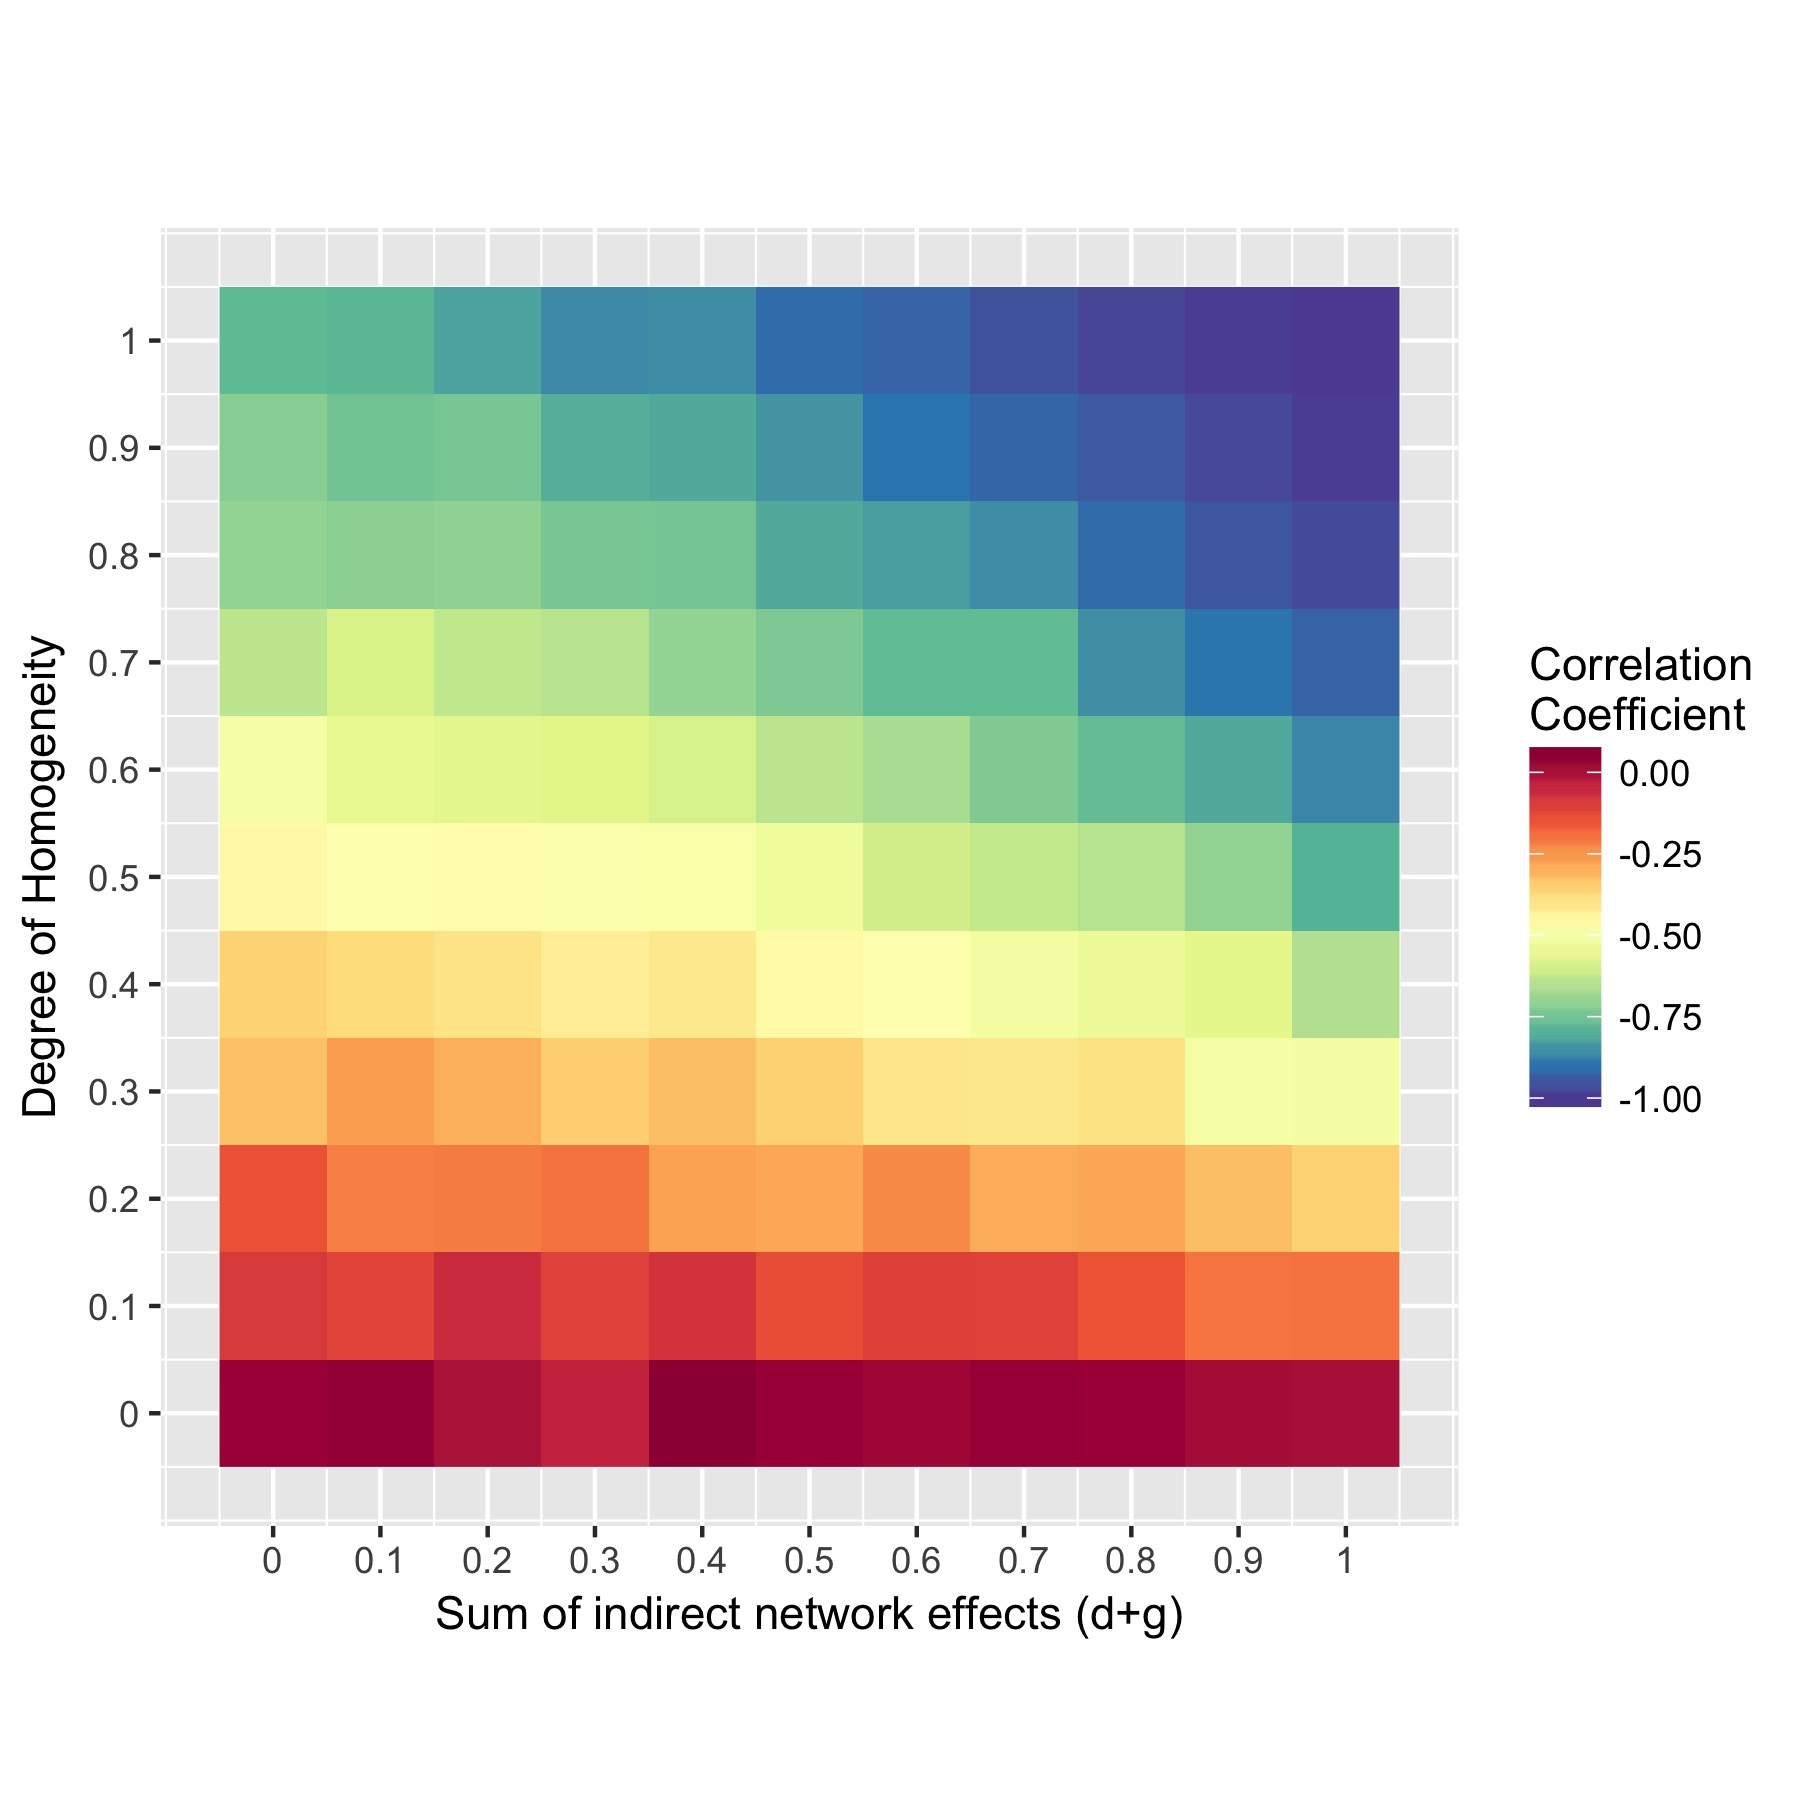
\includegraphics[width=.7\textwidth]{../figs/qqmatrix}
	\label{fig_QQa}
\end{figure}

\begin{figure}[H]
	\centering
	\caption{Simulated Correlation of $q_i$ and $q_j$ (b)}
	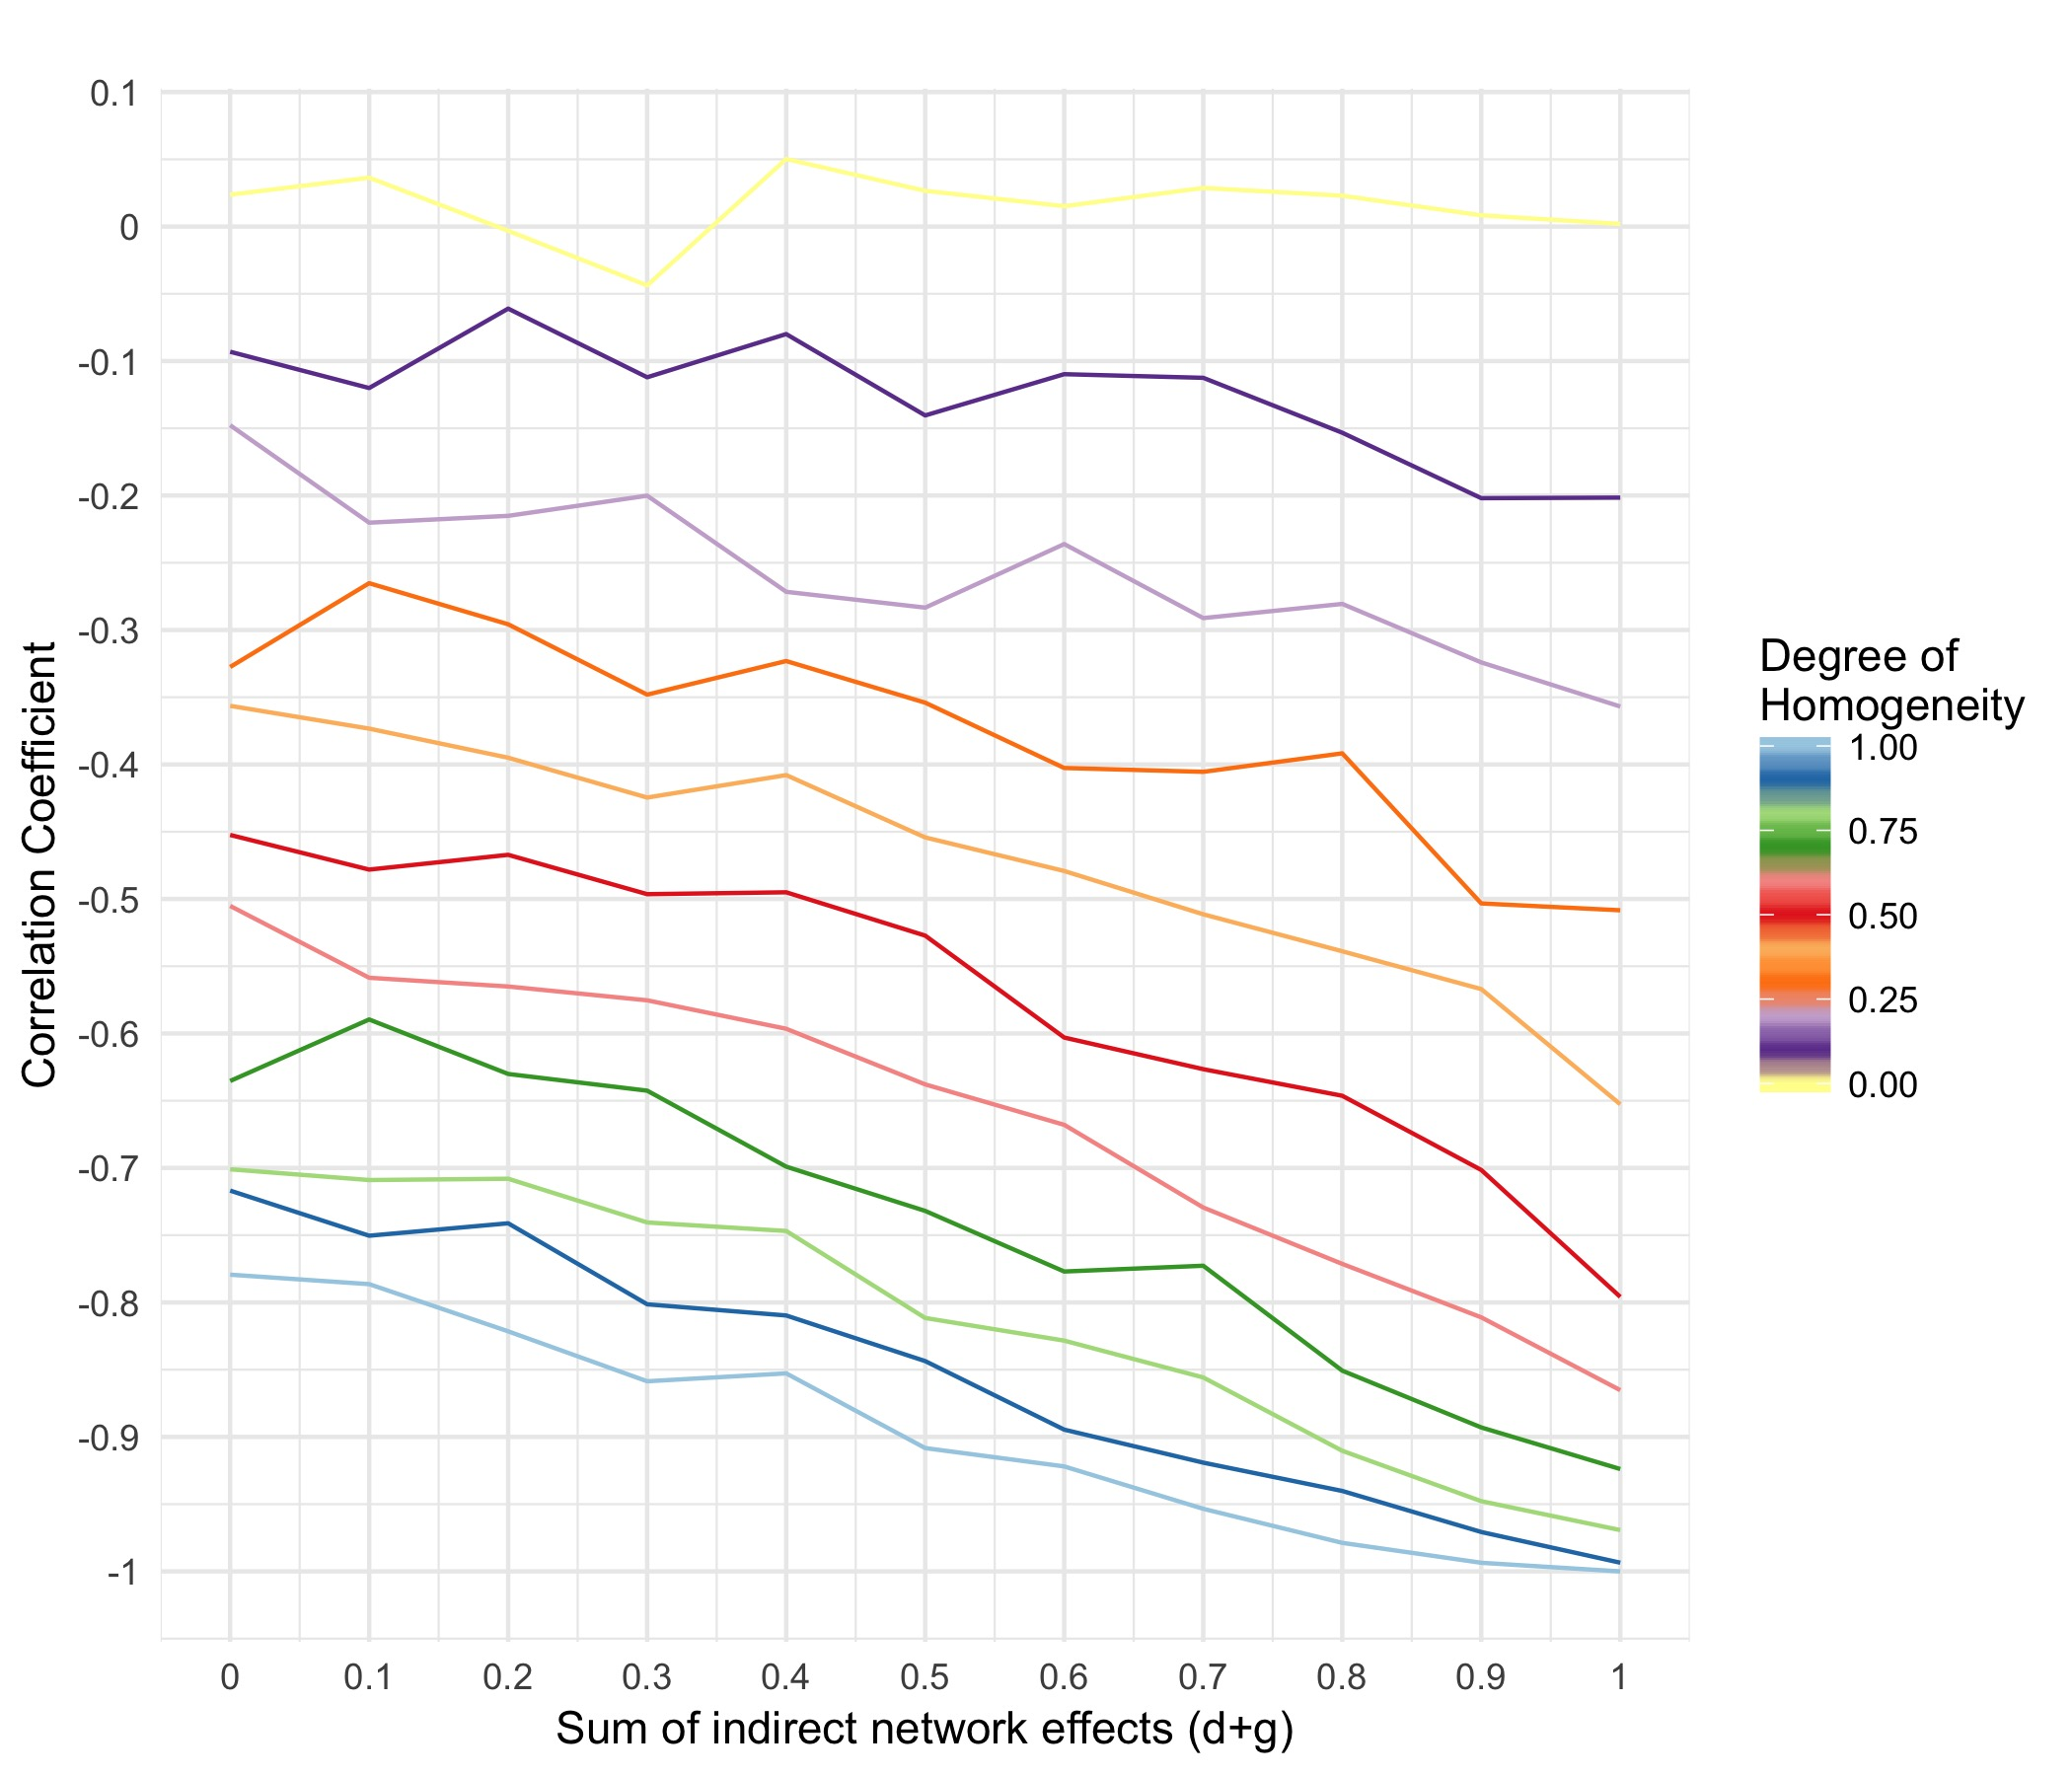
\includegraphics[width=.7\textwidth]{../figs/qqplot}
	\label{fig_QQb}
\end{figure}

% ----------------------------------------------------------------------------------------------------
%  EMPIRICAL ANALYSIS
% ----------------------------------------------------------------------------------------------------

\section{Empirical analysis}\label{empirical}

\subsection{A Simple method for detecting substitutional relationships in two-sided markets}

This section presents a simple method for detecting substitutional relationships in two-sided markets using cross-correlation functions and simple contemporary correlations. To test our approach to identifying substitutional relationships, we use data from popular German magazines, which are typical of two-sided markets. Magazine publishers serve a reader market and an advertising market, which are both interrelated by indirect network effects. Furthermore, data on German popular magazines is available for a broad range of differentiated products for both reader advertising markets. Therefore, we can identify possible substitutional products from a relatively high number of genres. Identification of possible substitutes has to be based on plausibility considerations. As popular magazines are typically highly differentiated, characteristics such as price level, layout, frequency of publication, and socio-demographic factors of readers can help identify possible competitors.  

As data from identical markets are typically affected by the same external influences, time series of prices and quantities are usually overlapped by common patterns. While quantities are strategic substitutes, we expect to find negative contemporary correlations between substitutes. However, quantities and prices set by platforms from the same market or industry typically show identical patterns, e.g., seasonality, expected trends, or cyclical behavior. In order to prevent spurious regressions, identical patterns have to be removed before an analysis of substitutability can be applied. For this purpose, we first apply different prewithening procedures. At first, we apply a method proposed by \cite{dewenter_essays_2004}. All series from similar markets which show the same patterns are regressed on each other, including a trend and a constant. Next, different time series models, such as ARMA and ARIMA models, are applied for pre-whitening matters (see \cite{box_time_2008}). The results from different models are used for comparison.

Next, we can calculate either simple correlation coefficients or cross-correlation functions and compare the results with simulated correlations. Using cross-correlation functions instead of simple correlation coefficients allows us to analyze contemporary correlation and possible effects such as shifts in quantities from one magazine to another. These shifts typically occur with the market entry of new products. Given that all competitors compete for a more extended period, contemporary correlation coefficients should be an adequate measure. 

\subsection{Data}\label{sec:data}

Data used in this study is extracted from the online magazine database ``PZ Online'' (Public Magazines Online), which provides (among other things) information on circulation, advertising volumes, and prices for a high number of magazines from different genres.\footnote{PZ Online is provided by the German association of magazine publishers (Verband Deutscher Zeitschriftenverleger) to provide advertising customers with necessary information on possible advertising platforms.} In order to address somewhat different genres and markets, we use data on news magazines as well as on women's and TV magazines. 

We use circulation numbers and advertising pages per copy to account for quantities in reader and advertising markets, respectively. 
Even though the dataset contains data from 2003 to date, we restrict our analysis to different two and three-year intervals (see Table \ref{t_sample selection} for an overview of our samples). The reasoning behind subsampling is two-fold: First, as data availability often plays a crucial role in any economic policy analysis, using shorter periods allows us to prove that our approach is suitable even with low data availability. 
Second, antitrust concerns are often related to specific periods as markets develop constantly. Additionally, during recent years, print media have been subject to decreasing circulation and declining advertising revenues due to digitalization.\footnote{For more information see \cite{cabyova_impact_2014} or \cite{picard_digitization_2011}} Using data on magazine products proves that also markets with either decreasing or increasing market volumes can be subject to our approach.

% ---------sample table 
\begin{table}[ht]\centering
	\caption{Sample Selection}
\begin{adjustbox}{width=\textwidth}	
\begin{tabular}{llllllll}
\hline 
	 Segment 	& Titles & & & Period &  & Frequency & Obs \\ \hline
	News magazines 		& FOCUS & Der Spiegel & Stern & 2004 / 33 & 2006 / 33 & weekly & 105 \\
	 &  &  &  & 2013 / 33 & 2015 / 33 & weekly & 105 \\ \hline
	TV magazines 			& TV Movie & TV Spielfilm & TV Digital & 2007 / 15 & 2011 /15 & biweekly & 79 \\ \hline
	Women's magazines	& Brigitte & Freundin & Für Sie & 2007 / 15 & 2011 /15 & biweekly & 79 \\ \hline
\end{tabular}
	\label{t_sample selection}
\end{adjustbox}
\end{table}

\subsubsection{News Magazines} 

First published in 1947 ``Der Spiegel'' had a monopoly on investigative journalism for a long time when Burda-Verlag entered the market in 1993 with a news magazine, FOCUS, claiming itself to be a close substitute to Der Spiegel. The latter instead opposed that FOCUS is an illustrative magazine similar to Stern, a magazine first published in 1946 by Gruner + Jahr \citep{kaltenhaeuser_abstimmung_2005}. All three magazines differ regarding their editorial concept. Der Spiegel mainly focuses on complex political and social issues, whereas FOCUS also covers more non-political topics such as health and fitness. Stern has been a simple illustrative magazine without any political appeal until the 60s. It then started to address current political topics \citep{vogel_populaere_1998}. Even though all three magazines have different editorial concepts, the readership of Der Spiegel, FOCUS and Stern does not differ significantly regarding their socio-demographic characteristics but their political orientation: While FOCUS is rather a conservative outlet, the coverage of Der Spiegel can be considered as left-wing. Stern, which reporting is less political, can be located somewhere in between (\citet{kaltenhaeuser_abstimmung_2005}). Having this in mind, we do not expect strong competition in the reader market between the magazines as, e.g., a "left-wing" reader of Der Spiegel would probably not consider FOCUS as an adequate substitute et vice versa.\footnote{However as some of the readers might not have strong political preferences, we expect some kind of contemporary negative correlation, as cover stories and content will influence final purchasing decisions. This assumption is supported by the fact that subscription is just a minor part of total sales (about 2-3 $\%$). We assume, if any, weak negative indirect network effects from the advertising market as the share of advertising pages per copy ranges between 2$\%$ and 8$\%$.} All three magazines offer several digital services (website and mobile apps) with mostly free content. 

Advertising demand, on the other side, is assumed to be strongly affected by the size and the characteristics of the readership of a particular magazine. However, in contrast to the reader market, political orientation should not matter as much as socio-demographic characteristics. We, therefore, expect the degree of substitutability to be higher in the advertising market. All of the magazines might therefore be competitors in the advertising market.  

Visual inspection of the time series (see figure \ref{fig_fss}) shows that in the reader market, Stern and Der Spiegel have similar sales, whereas circulation of FOCUS is considerably smaller in both time samples. The overall mean decreased between the two periods by approximately 46$\%$, but sales of Der Spiegel were highest in both samples. Prices per copy remained the same without fluctuations, with Der Spiegel being more expensive ($4.6 EUR$) than FOCUS and Stern, who charge the same price per copy ($3.9 EUR$). On the advertising market, quantities of all three magazines are pretty similar and show seasonal fluctuations reveals, that the advertising pages of Der Spiegel are the lowest in terms of absolute and total values for both samples. Nevertheless, the standard deviation is relatively high, indicating a high fluctuation. Again, average quantities diminished between the time samples for both absolute and relative values. Looking at the prices per advertising side in the later sample shows that prices for Der Spiegel are highest, followed by Stern and FOCUS.\footnote{There is no publicly available data on advertising prices before 2009. However, available data shows an increase in advertising prices from 2009 to 2016.}

\begin{figure}[H]\centering
 \begin{center}
    \begin{subfigure}[normla]{0.49\textwidth}
        \includegraphics[scale=.5]{figs/sales_fss.pdf}
        \caption{Reader Market}
    \end{subfigure}
    \begin{subfigure}[normla]{0.49\textwidth}
        \includegraphics[scale=.5]{figs/ads_fss.pdf}
        \caption{Advertising Markt}
    \end{subfigure}
 \end{center}
\caption{Time Series of news magazines}
	\subfloat[Reader Market]{\includegraphics[scale=.3]{../figs/sales_fss}}
	\subfloat[Advertising Markt]{\includegraphics[scale=.3]{../figs/ads_fss}}
	\label{fig_fss}
\end{figure}


% ----------------------------
% ----- Programm Guides -----
% ----------------------------

\subsubsection{Program Guides}

In contrast to the market for news magazines, the market for program guides consists of a relatively high number of magazines. However, the market is also strongly segmented into different sub-markets (e.g., weekly and bi-weekly, high price, and low price). In order to test our model, we chose a segment of bi-weekly magazines characterized by similar presentation, layout, and content. A presumably high degree of substitutability can also be suspected from similar titles: TV Spielfilm, TV Movie, and TV Today.  

Visual inspection confirms our suspicion that these are substitute products. Overall sales vary in absolute terms (see Figure \ref{fig_tv}), but all magazines in our sample show similar trends and peaks. While TV Spielfilm and TV Movie show similar fluctuations and levels across the sample, TV Today appears to trend somewhat differently. However, sales volatility is much lower compared to the news magazines. There are also more significant fluctuations in advertising revenues, which show a similar trend.  


\begin{figure}[H]\centering
\caption{Time Series of program guides}
	\subfloat[Reader Market]{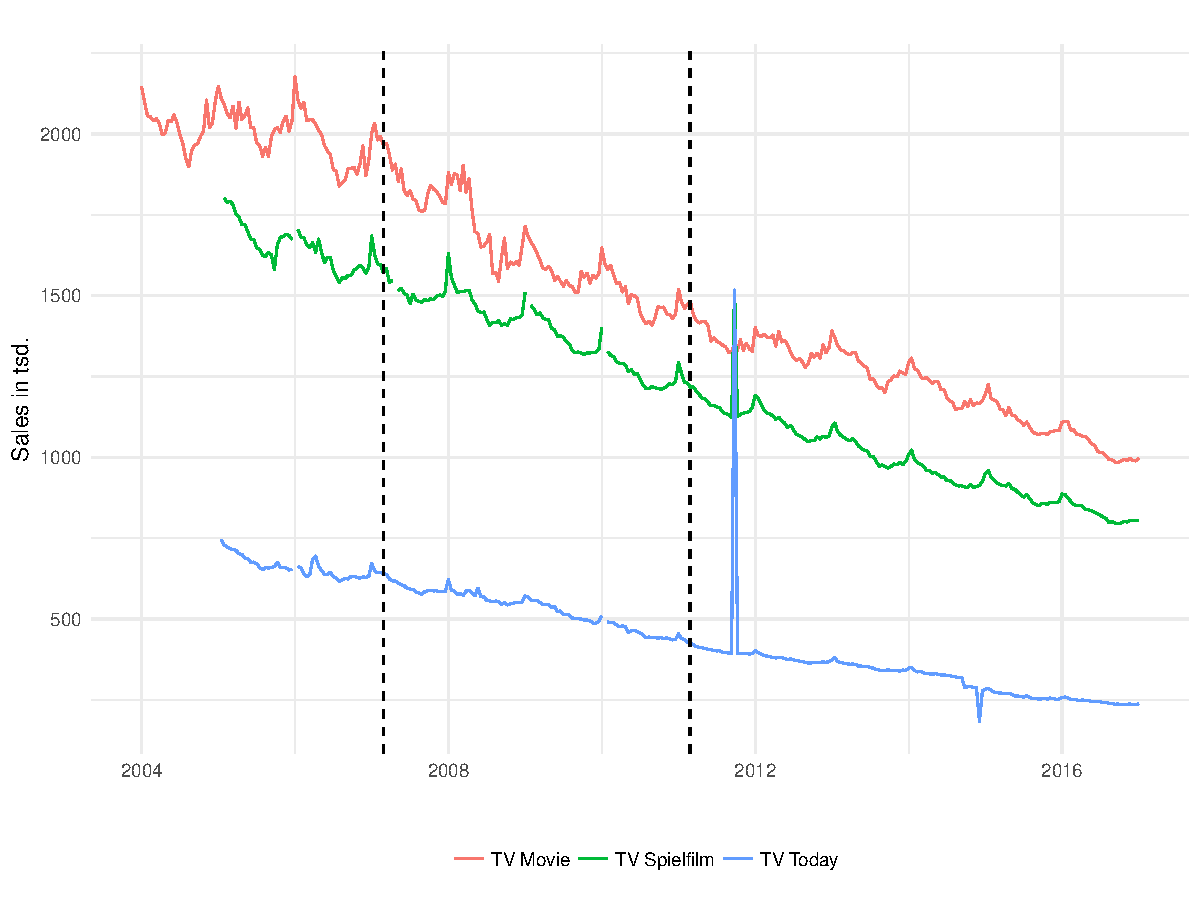
\includegraphics[scale=.3]{../figs/sales_tv}}
	\subfloat[Advertising Markt]{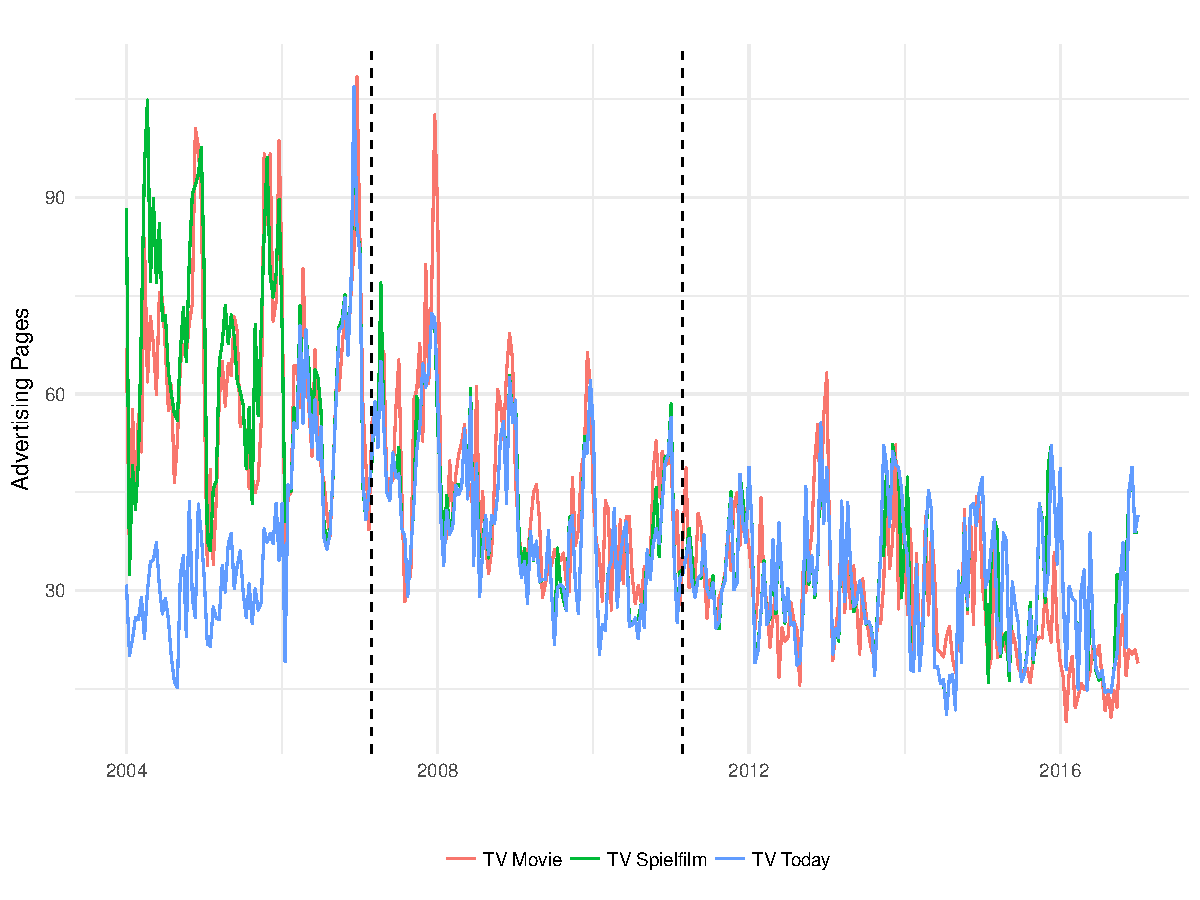
\includegraphics[scale=.3]{../figs/ads_tv}}
	\label{fig_tv}
\end{figure}


\subsubsection{Women's magazines}
\todo{state new results}

Women's magazines are the most popular journals in Germany and are highly differentiated. While some magazines are located in a low price segment, others represent a glossy high price section. Journals are also differentiated with respect to content, resulting in a high number of different products, focussing on topics such as fashion, beauty, gossip, and others. To test the validity of our approach, we chose the three magazines Brigitte, Freundin, and Für Sie, all of them published biweekly, showing similarities regarding editorial content and copy price. The three magazines cover topics such as fashion, beauty, health, and nutrition and reportage on particular topics to reach the target audience of middle-aged women. Copy prices range between 2.9EUR (Für Sie) and 3.2EUR (Brigitte) and do not show any fluctuations from 2003 to 2016.\footnote{Copy price of Freundin is 3EUR.} 

Inspecting time series plots of sales and advertising pages (see figure \ref{fig_women}) reveals relatively high sale numbers for Brigitte and quite lower sales for Freundin and Für Sie. All series on sales are more volatile than series on TV magazines, probably because demand for women's magazines may depend on current coverage to a much higher degree. Advertising space is also volatile and characterized by seasonal fluctuation, which affects all of the times series similarly. However, advertising volumes are smaller for Freundin. Again, the quantities on both market sides do not indicate negative correlations. However, as the time series seem to follow a common structural trend, the assumption of a substitutional relationship is reasonable. 


\begin{figure}[H]\centering
\caption{Time Series of women magazines}
	\subfloat[Reader Market]{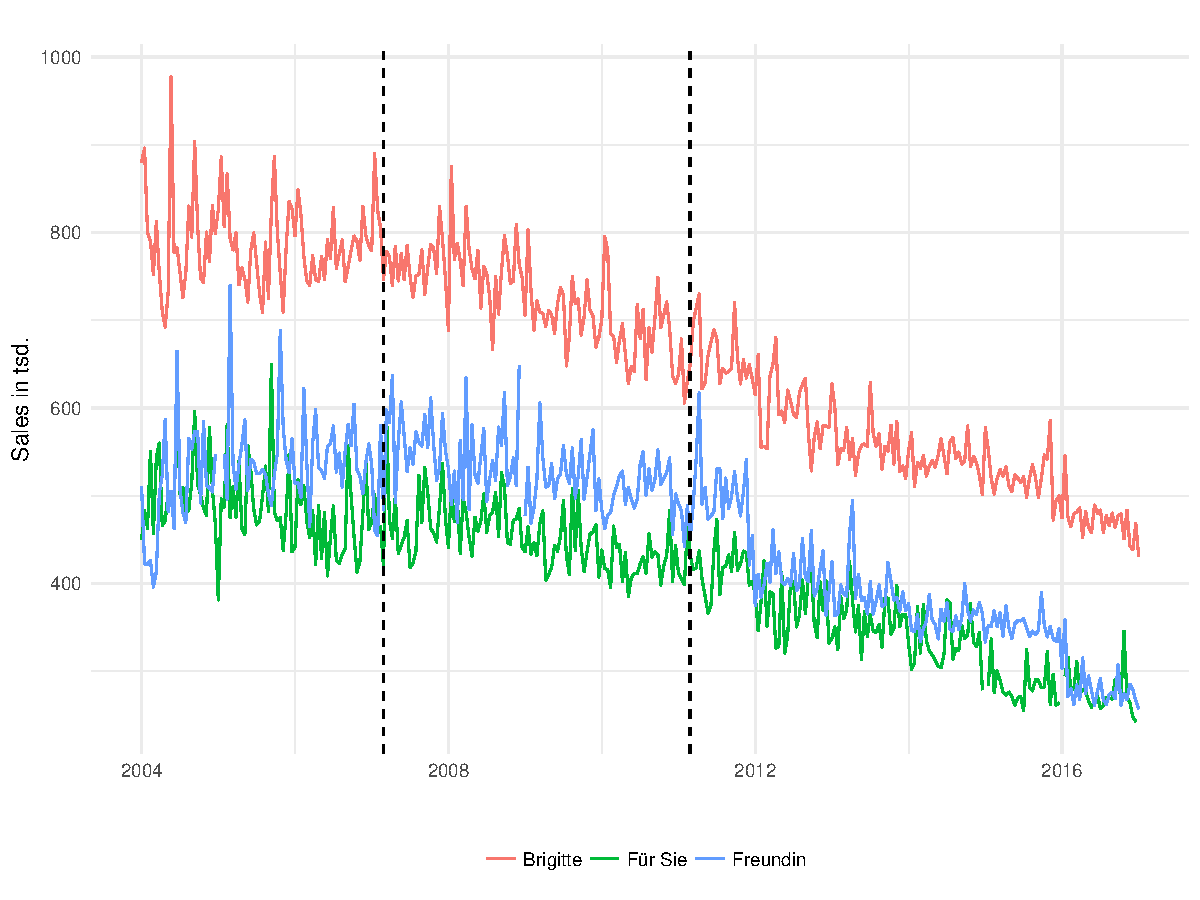
\includegraphics[scale=.3]{../figs/sales_women}}
	\subfloat[Advertising Markt]{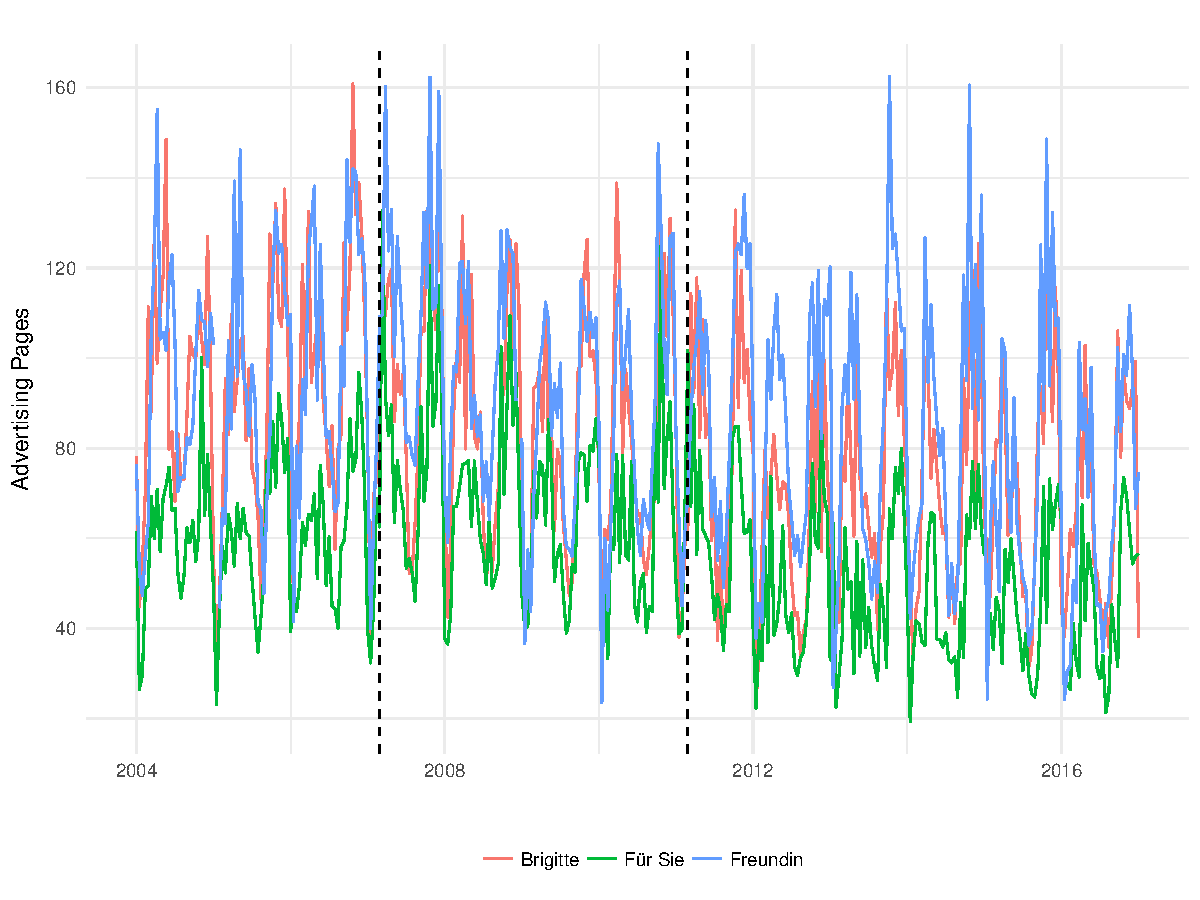
\includegraphics[scale=.3]{../figs/ads_women}}
	\label{fig_women}
\end{figure}


% ----------------------------------------------------------------------------------
% RESULTS
% ----------------------------------------------------------------------------------

\subsection{Results}

\subsubsection{News magazines}

To prevent a possible spurious regression, all-time series have first been analyzed for non-stationarity using Philipps-Perron unit roots tests. As can be seen from the results in the appendix, all of the series are of order I(0). Next, different pre-whitening procedures have been applied as described above to produce adjusted time series that are adequate for correlation analysis. Figures \ref{fig_arima_sales_fss} and \ref{fig_arima_ads_fss} present adjusted series using the appropriate ARMA process for both markets and periods. Time series are therefore adjusted for common trends and other structural components. A spurious regression should therefore be excluded.  

\subsubsection{Reader Market}

Next, we analyze the reader market for news magazines by calculating cross-correlation functions using adjusted time series for sales. As figure \ref{fig_ccf_sales_fss} shows,\footnote{(1) = 2004w33-2006w33, (2) = 2013w33-2015w33} relatively small contemporary correlation coefficients exist, indicating (if any) only weak substitutional relationships between the magazines.\footnote{Note that $t<0$ indicates the correlation between the current sales of the first magazine and the lagged sales of the second magazine. The dashed lines represent the respective approximated two standard error bounds $SE^+=\frac{2}{\sqrt{n}}$ and $SE_-=\frac{-2}{\sqrt{n}}$ \citep{tiao_modeling_1981}.} For the first period no significant contemporary correlation can be found.\footnote{Corresponding contemporary values can be found in table \ref{tab_CCF}} For the second period a slightly stronger correlation indicating a weak substitutional relationship between Der Spiegel and Stern ($\rho=-0.30$) is evident.

\begin{figure}[H]
\caption{CCF sales}
	\centering
	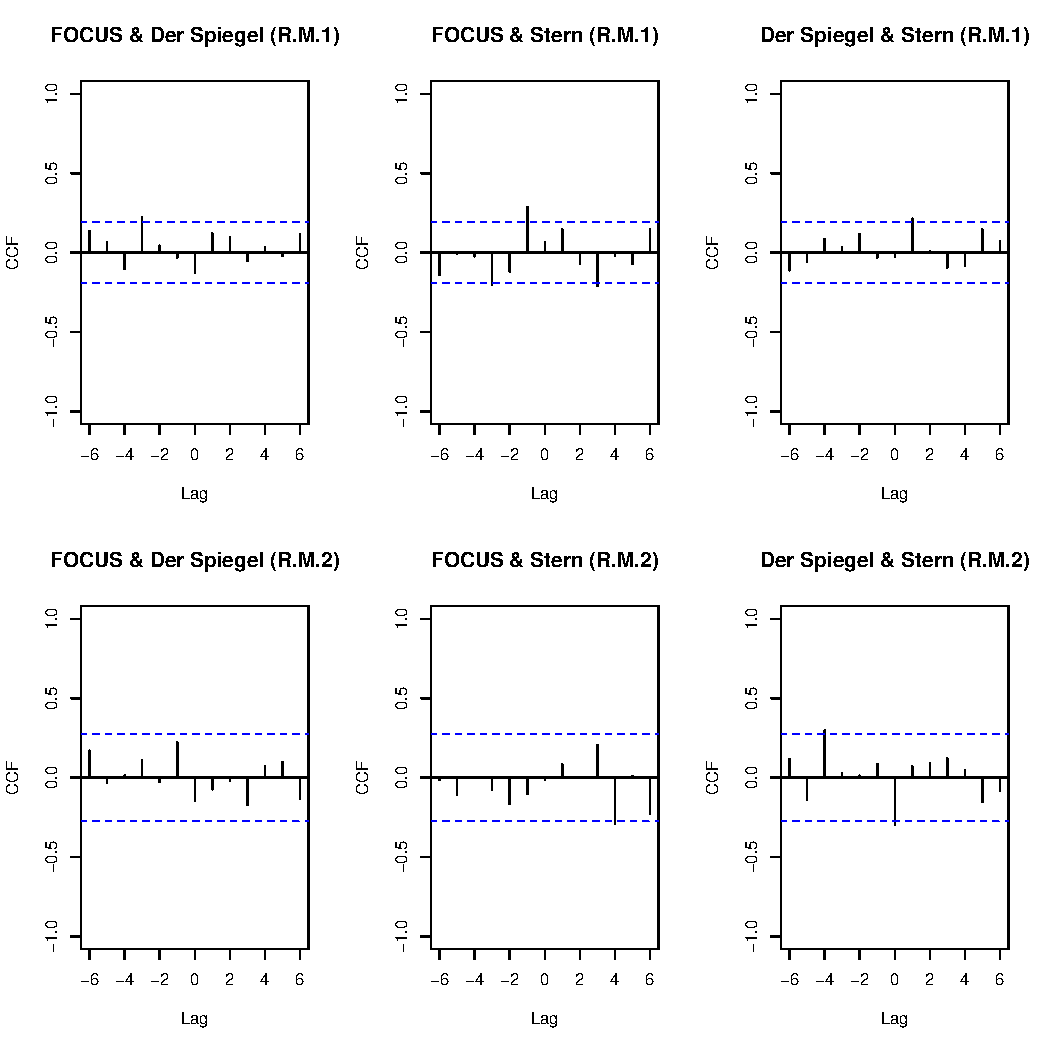
\includegraphics[scale=0.5]{../figs/ccf_sales_fss}
	\label{fig_ccf_sales_fss}
\end{figure}

\subsubsection{Advertising Market}
Turning to the advertising market, figure \ref{fig_ccf_ads_fss} supports the assumption that competition on this market side is much stronger. In contrast to the reader market, all contemporary correlations are statistically significant and negative. In the first sample, we can find a substitutional relationship among all three magazines, with a contemporary negative correlation of $\rho=-0.53$ for FOCUS \& Der Spiegel being the strongest. Der Spiegel \& Stern show a rather weak substitutional relationship ($\rho=-0.38$), and a contemporary correlation for FOCUS \& Stern of $\rho=-0.43$. In the second period, competition seems to have decreased between FOCUS \& Stern, as the correlation coefficient is $\rho=-0.32$. Contemporary correlation between Der Spiegel \& FOCUS ($\rho=-0.53$) and FOCUS \& Stern ($\rho=-0.38$) did not change significantly. It is striking that some of the intertemporal effects of FOCUS \& Stern are positive and significant. This phenomenon might be due to a common trend that has not been filtered in the first stage. Because of the weekly data, a separated seasonal adjustment could only be carried out with an enormous effort, as irregular effects such as calendar effects or moving festivals appear within the time series (\cite{harvey_modeling_1997}). Such common structural trends are assumed to have a positive rather than a negative influence on the results. 

\begin{figure}[H]
\caption{CCF advertising pages/copy}
	\centering
	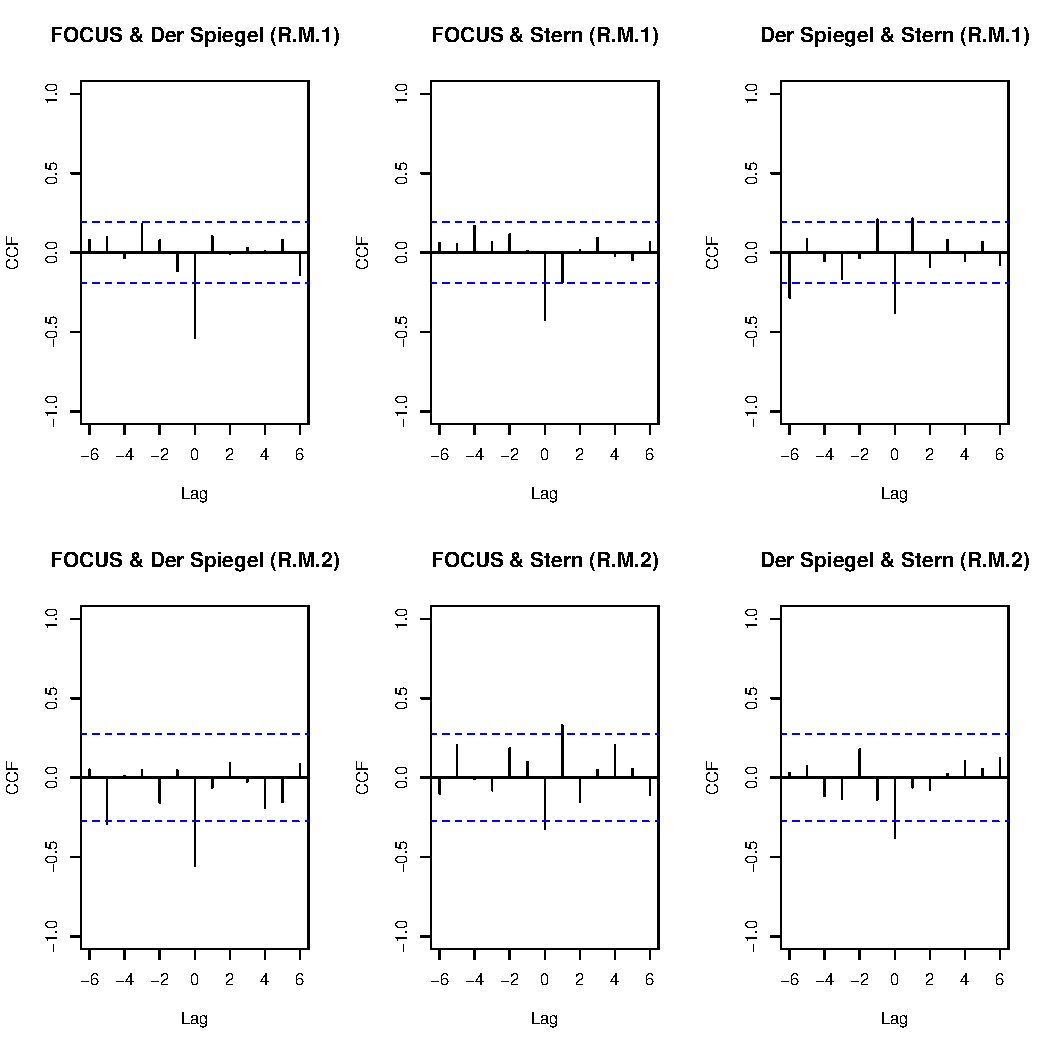
\includegraphics[scale=0.5]{../figs/ccf_ads_fss}
	\label{fig_ccf_ads_fss}
\end{figure}

\begin{table}[!htbp] \centering
	\caption{Contemporary correlations}
	\label{tab_CCF}
\begin{tabular}{@{\extracolsep{5pt}} lll}
\\[-1.8ex]\hline 
\hline \\[-1.8ex]
	news magazines(1) & sales & ad pages/copy \\
	\hline
	FOCUS \& Der Spiegel & -.124 & -.534 \\
	FOCUS \& Stern & .068 & -.426 \\
	Der Spiegel \& Stern & -.027 & -.377 \\
	\hline
	news magazines(2) & & \\
	\hline
	FOCUS \& Der Spiegel & -.147 & -.553 \\
	FOCUS \& Stern & -.012 & -.322 \\
	Der Spiegel \& Stern & -.296 & -.379 \\
	\hline
	program guides & & \  \\ 
	\hline
	TV-Spielfilm \& TV-Movie & -.078 & .059 \\
	TV-Spielfilm \& TV-Today & -.735 & -.953 \\
	TV-Movie \& TV-Today & -.071 & -.223 \\ 
	\hline
	women's magazines &  & \  \\ 
	\hline
	Brigitte \& Für Sie & -.490 & -.366 \\ 
	Brigitte \& Freundin & -.090 & -.414 \\ 
	Für Sie \& Freundin & -.240 & -.530 \\ \hline
\end{tabular}
	\end{table}

\subsubsection{Comparison with Benchmark}

Figure \ref{fig_QQ_fss} shows the estimated contemporary correlation of news magazines for the second sample (2013/33-2015/33) compared with the simulated benchmark.\footnote{F=FOCUS, DS=Der Spiegel, S=Stern.} Assumptions about the amount of INE change the indicated degree of competition: The higher the assumed sum of INE, the lower is $\theta$. In other words, the same negative correlation coefficients indicate less competition if the INE is high. Assuming that total INE (from reader market to advertising market and reverse) exist and are positive, the following conclusions can be drawn: In the reader market, no significant contemporary correlation coefficients were found in the first sample. In the later sample, the substitutional relationship between Der Spiegel and Stern intensified ($\rho\approx0.3$), indicating a degree of competition of $\theta\approx0.3-0.4$ depending on the assumed INE.

Turning to the advertising market, the substitutional relationship between FOCUS and Der Spiegel is the strongest for both samples. If we assume that the sum of INE ranges between 0 and 0.3, we can find a degree of homogeneity of nearly $\theta\approx0.7$, whereas the INE of 0.7 to 0.9 indicates $\theta\approx0.5-0.6$. Negative correlation between FOCUS \& Stern decreased between the samples (from $\rho=-0.43$ to $\rho=-0.32$), suggesting a degree of homogeneity of $\theta\approx0.3$ for the later sample (or $\theta\approx0.2$ if we assume $d+g>0.9$). The substitutional relationship between Der Spiegel \& Stern did not change significantly between the two samples, indicating a degree of homogeneity of $\theta\approx0.4-0.5$.


\begin{figure}[H]\centering
\caption{cross-correlation / news magazines}
\subfloat[reader market]{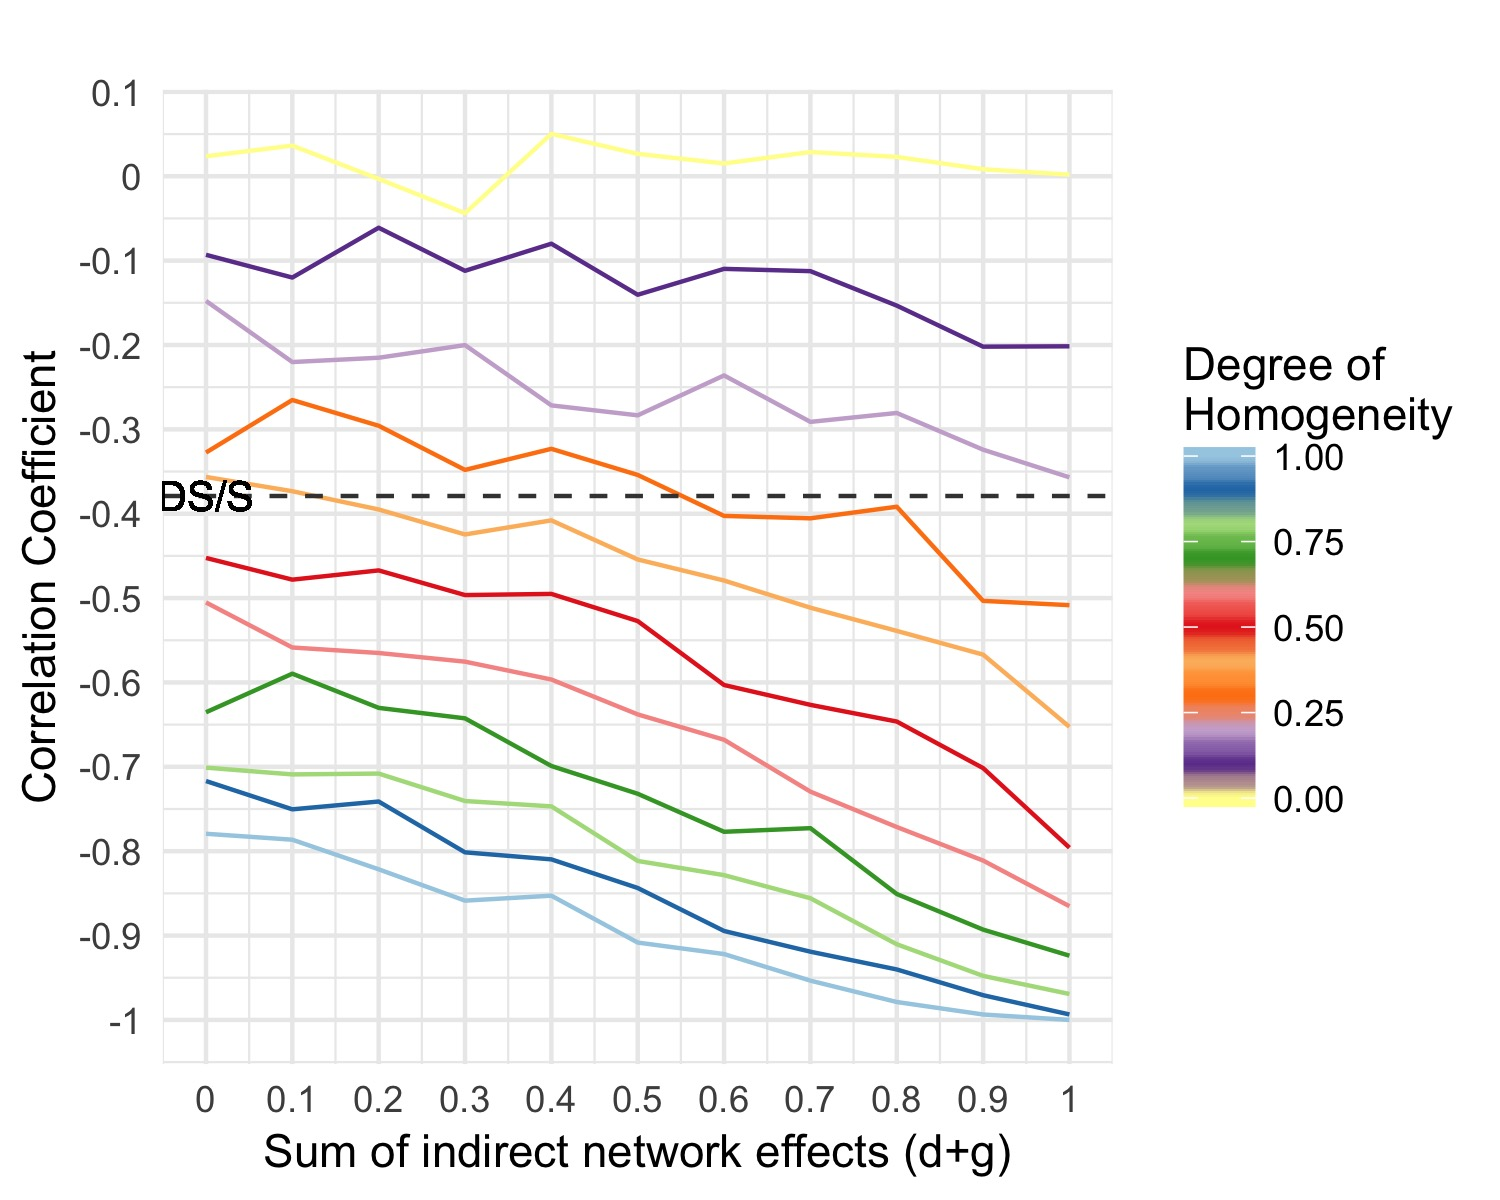
\includegraphics[width=0.5\textwidth]{../figs/qq_sales_fss}}
\subfloat[advertising market]{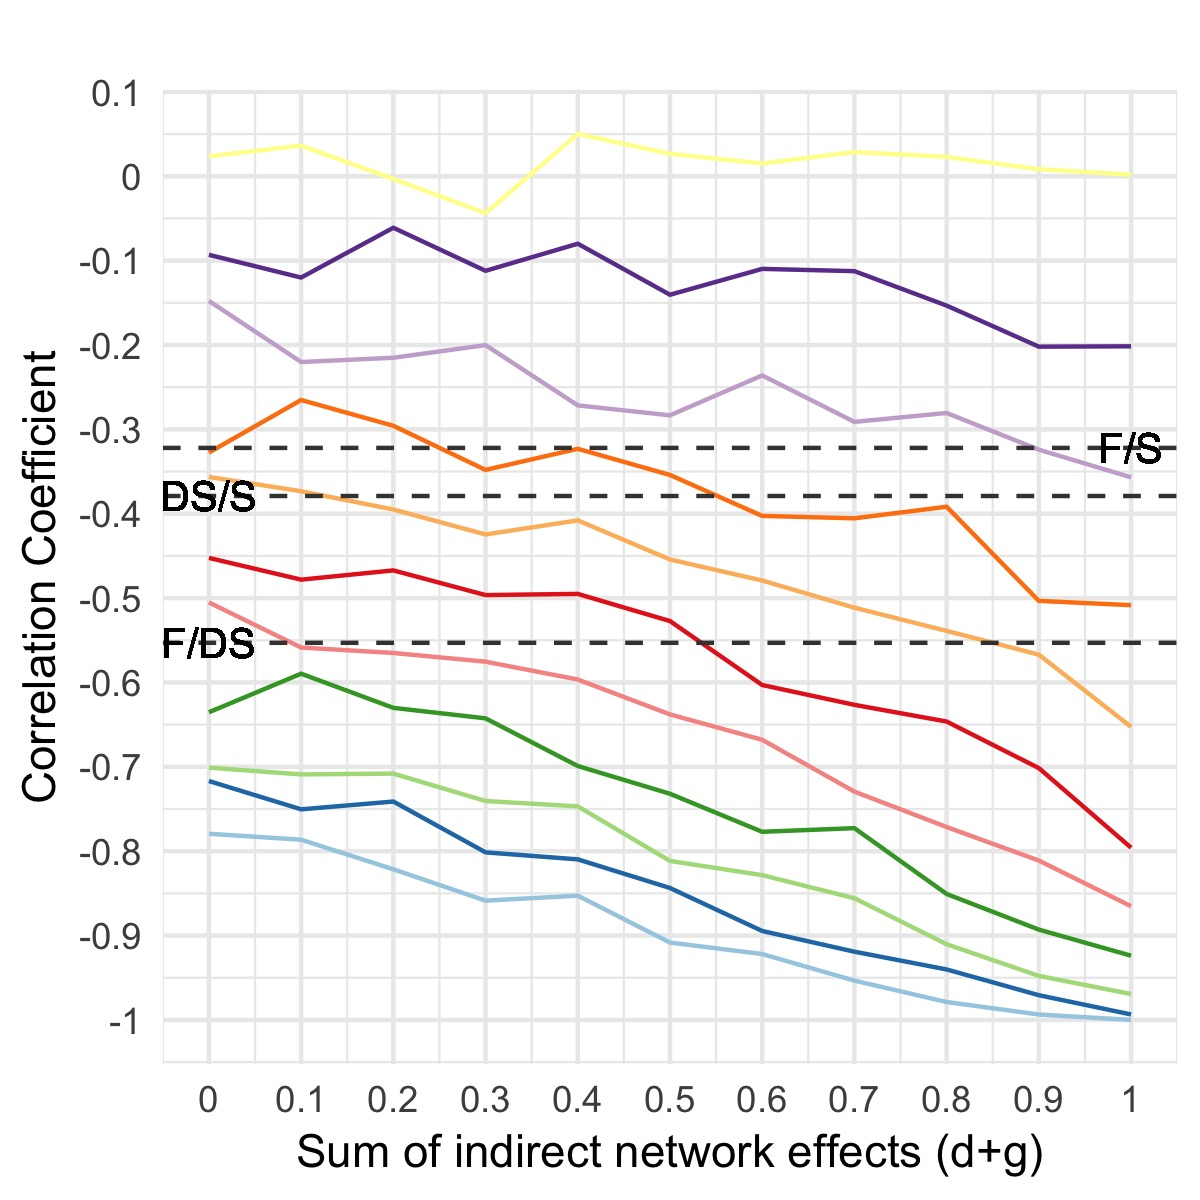
\includegraphics[width=.4\textwidth]{../figs/qq_ads_fss}}
\label{fig_QQ_fss}
\end{figure}

Our empirical results imply much stronger substitutional relationships in the advertising market for all pairs of magazines. These results strongly support the assumption of the dichotomy of the two market sides with respect to a market definition. Furthermore, the contemporary correlation in the advertising market increased between the two periods for FOCUS and Stern, whereas no significant change was found for the remaining two pairs. The degree of competition between the last two pairs can be assumed to have remained the same. 

Contemporary substitutional relationships increased between the periods regarding Der Spiegel \& Stern, turning to the reader market. This might be due to a change in the editorial concept of one or both magazines. No significant substitutional relationship was found for the other pairs in both samples. 

Overall, the empirical results support the assumption that the three magazines are substitutes in the advertising market but seem to claim their own sub-markets in the reader market within both periods. 

\subsubsection{Program Guides}

A similar analysis has been conducted for the market of program guides, including the magazines TV-Movie, TV-Spielfilm, and TV-Digital. 
Again, unit root tests and time pre-whitening have been carried out as a first step. Figure \ref{fig_arima_tv} includes adjusted time series for all TV magazines from both markets.  

Figure \ref{fig_ccf_tv} shows the cross-correlation functions of the reader (R.M.) and the advertising market (A.M.). The magnitude of the contemporary correlation between TV-Today and TV-Spielfilm is the strongest on both market sides (with $\rho=-.74$ in the reader and $\rho=-.95$ in the advertising market, respectively). Comparing these results with our benchmark model and assuming positive INE, the competition parameter ranges between $\theta\approx.9-.6$ in the reader market and $\theta\approx1-.75$ in the advertising market. Again, the degree of competition depends on the sum of the indirect network effects: the higher the assumed INE, the lower the competition parameter for the same correlation coefficient. Contemporary correlations in the advertising market between TV-Movie and TV-Today are statistically significant but relatively small in the reader market $\rho=-.22$, indicating degrees of substitutability of $\theta\approx.15$. No significant correlation can be found between TV-Spielfilm and TV-Movie.

\begin{figure}[H]
\caption{CCF program guides}
	\centering
	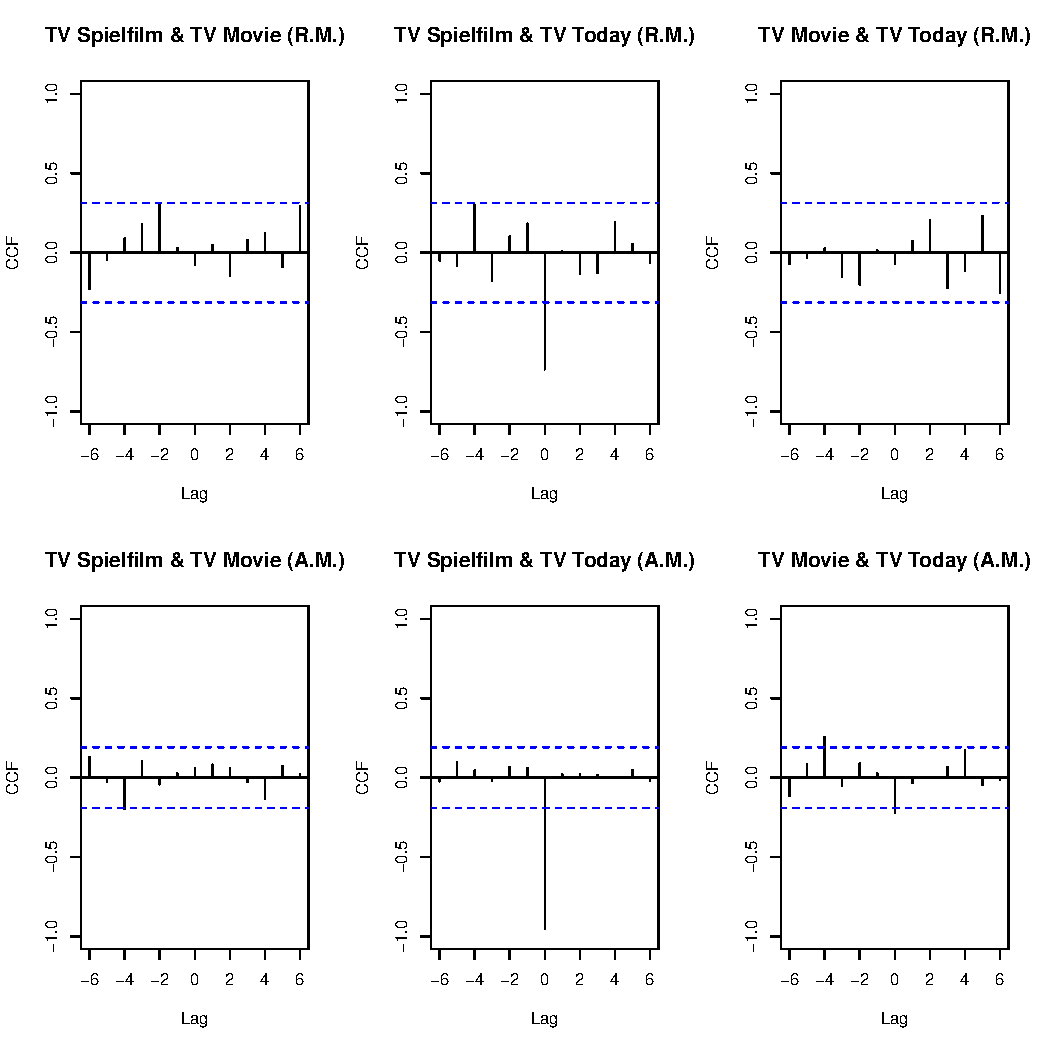
\includegraphics[scale=0.5]{../figs/ccf_tv}
	\label{fig_ccf_tv}
\end{figure}

\subsubsection{Women's Magazines}

The ccf of the adjusted time series are shown in figure \ref{fig_ccf_women}. As a striking outcome, the contemporary correlation between Brigitte \& Für Sie is higher in the reader market ($\rho=-.49$, suggesting a degree of homogeneity of $\theta\approx.4-.5$) than in the advertising market ($\rho=-.37$, suggesting a degree of homogeneity of $\theta\approx.3-.43$). The contemporary correlation between Brigitte \& Freundin is insignificant in the reader market but suggests a substitutional relationship in the advertising market ($\rho=-.41$ leads to $\theta\approx.3-.4$). Für Sie \& Freundin show an even higher correlation on the reader market ($\rho=-.53$), indicating a degree of competition of $\theta\approx0.4-0.5$, whereas on the reader market, these magazines seem to be only weak substitutes ($\rho=-.24$ leads to $\theta \approx .15$).

Put differently, women's magazines seem to be closer substitutes in the advertising than in the reader market. Although this may seem counter-intuitive, this result is typical for some media markets. As described above, even if different groups of readers do not consider some specific media outlets as substitutes, this does not necessarily imply that advertising customers do not consider the magazines' readerships as substitutional. 

\begin{figure}[H]
\caption{CCF women's magazines}
	\centering
	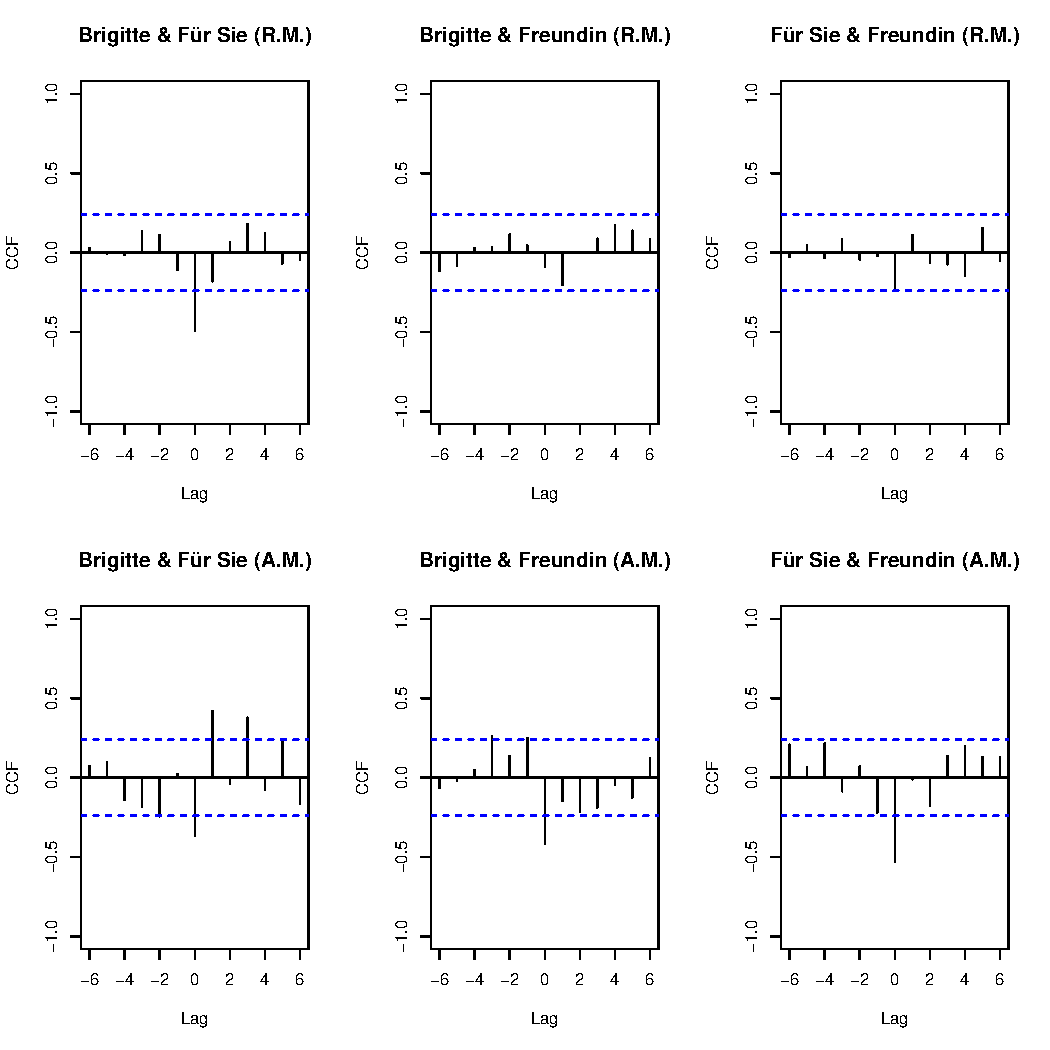
\includegraphics[scale=0.5]{../figs/ccf_women}
	\label{fig_ccf_women}
\end{figure}

\subsubsection{Program guides and women's magazines }

In order to test the validity of our method, we finally calculated cross-correlation functions between women's magazines and TV guides. As expected, there is no evidence for any significant substitutional relationship. Neither for the reader nor the advertising market are any statistically significant correlations to be found. This result is, of course, not surprising at all, as TV guides and women's magazines cannot be considered substitutes in the reader market. A similar logic applies to the advertising market. Although there might be some products for which advertising customers consider TV guides and women's magazines as possible advertising outlets, the readerships of both types of magazines are supposed to be quite different regarding socio-demographic characteristics. However, socio-demographics are most important for identifying advertising customers' target groups.

\begin{figure}[H]
\caption{CCF women's magazines and program guides}
\label{ccf_tvfrauen}
	\centering
	\includegraphics[width=.9\textwidth]{ccf_tvfrauen.eps}
\end{figure}

\section{Conclusions}

Market definition in two-sided markets is a complex challenge, and until now, no method has been developed which is applicable and suitable as a practical antitrust tool. Usual methods developed for on-sided markets are no longer valid, and the interdependence of quantities and prices from both markets, caused by indirect network effects, leads to severe identification problems. For this reason, some authors recommend altogether abandoning the market definition as it is considered useless and incoherent \citep{noel_analyzing_2005, kaplow_market_2014}. However, competition authorities are either obliged to define markets or have at least to identify the closest competitors to evaluate the effects of possibly anti-competitive behavior.     

For this reason, we developed a new method for identifying competitors in two-sided markets by using time series methods and simple correlation analysis. At first, time series on quantities from both markets are adjusted by time series models to prevent spurious regressions. We use quantities instead of prices as (i) substitutability is directly reflected in quantities but not necessarily in prices; (ii) indirect network effects are directly linked to quantities and (iii) two-sided markets, such as platform markets typically characterized by zero prices on either of the submarkets. Next, either cross-correlation functions or simple contemporary correlations are calculated to identify the substitutability of different products. The procedure is applied to the reader and advertising markets of different popular magazines genres. 

To evaluate the degree of substitutability between different media outlets, we first build a simple model of two-sided markets. We then use Monte Carlo simulations to calculate correlation coefficients for varying degrees of product differentiation and indirect network effects. A comparison of empirical correlations with Monte Carlo results can then be used to identify the degree of substitutability. 

The conclusions from our empirical analysis is twofold: First, our method seems to be appropriate to estimate degrees of substitutability in two-sided markets. The results seem to be reasonable and valid. Correlation coefficients are surprisingly different between seemingly similar products. This applies especially to circulation. 

The conclusions from our empirical analysis are twofold: First, our method seems to be appropriate for estimating degrees of substitutability in two-sided markets. The results seem reasonable and valid, as correlation coefficients are surprisingly different between seemingly similar products,  especially in circulation. Second, our analysis shows that market definition is likely to be asymmetric between different markets (i.e., the reader and the advertising market). While circulation between most products shows only moderate substitutability, correlations in the advertising market seem to be much higher. These results are also in line with our theoretical considerations. 

As we have analyzed only a small number of magazines, the next step is to include a much higher number of outlets from different segments. Especially online platforms markets are interesting research objects, as many recent antitrust cases affect digital platforms. \pagebreak

% ----------------------------------------------------------------------------------------------------
%  APPENDICES
% ----------------------------------------------------------------------------------------------------

\printbibliography \pagebreak

\begin{appendices}

\section{Empirical analysis}

\subsection{Phillips-Perron test for unit Root}

%%%%%%%%%%%%% Without Trend %%%%%%%%%%%%%%%

\begin{table}[!htbp]\centering 
  \caption{Unit Root Test, no trend} 
  \label{tab_uroot} 
\begin{tabular}{@{\extracolsep{5pt}} llll} 
\\[-1.8ex]\hline 
\hline \\[-1.8ex] 
 & FOCUS & Der Spiegel & Stern \\ 
\\[-1.8ex]\hline 
\hline \\[-1.8ex] 
2004 - 2006 \\
\hline
Sales & -8.20 & -5.27 & -6.01 \\ 
Ad pages & -3.49 & -3.33 & -3.60 \\ 
\hline
2013 - 2015 \\
\hline
Sales & -10.69 & -7.63 & -8.51 \\ 
Ad pages & -3.83 & -4.50 & -4.99 \\ 
\hline
Sig. Level & 1pct & 5pct & 10pct \\ 
Critical Values & -3.49 & -2.89 & -2.58 \\ 
%%%%%%% Program Guides 
\\[-1.8ex]\hline 
\hline \\[-1.8ex] 
 & TVMovie & TVSpielfilm & TVDigital \\ 
\\[-1.8ex]\hline 
\hline \\[-1.8ex] 
Sales & -0.02 & -0.15 & -1.66 \\ 
Ad pages & -4.14 & -4.34 & -5.74 \\
\hline 
Sig. Level & 1pct & 5pct & 10pct \\ 
Critical Values & -3.52 & -2.90 & -2.9 \\ 
%%%%%%% Womens Magazines  
\\[-1.8ex]\hline 
\hline \\[-1.8ex] 
 & Brigitte & Freundin & Für Sie \\ 
\\[-1.8ex]\hline 
\hline \\[-1.8ex] 
Sales & -5.96 & -7.87 & -4.66 \\ 
Ad pages & -4.87 & -4.15 & -5.26 \\ 
\hline
Sig. Level & 1pct & 5pct & 10pct \\ 
Critical Values & -3.52 & -2.90 & -2.59 \\ 
\hline \\[-1.8ex] 
\end{tabular} 
\end{table} 

\subsection{Adjusted Time Series}

\begin{figure}[H]
		\caption{Sales of news magazines (adjusted)}
		\centering
		\subfloat[Sample 1]{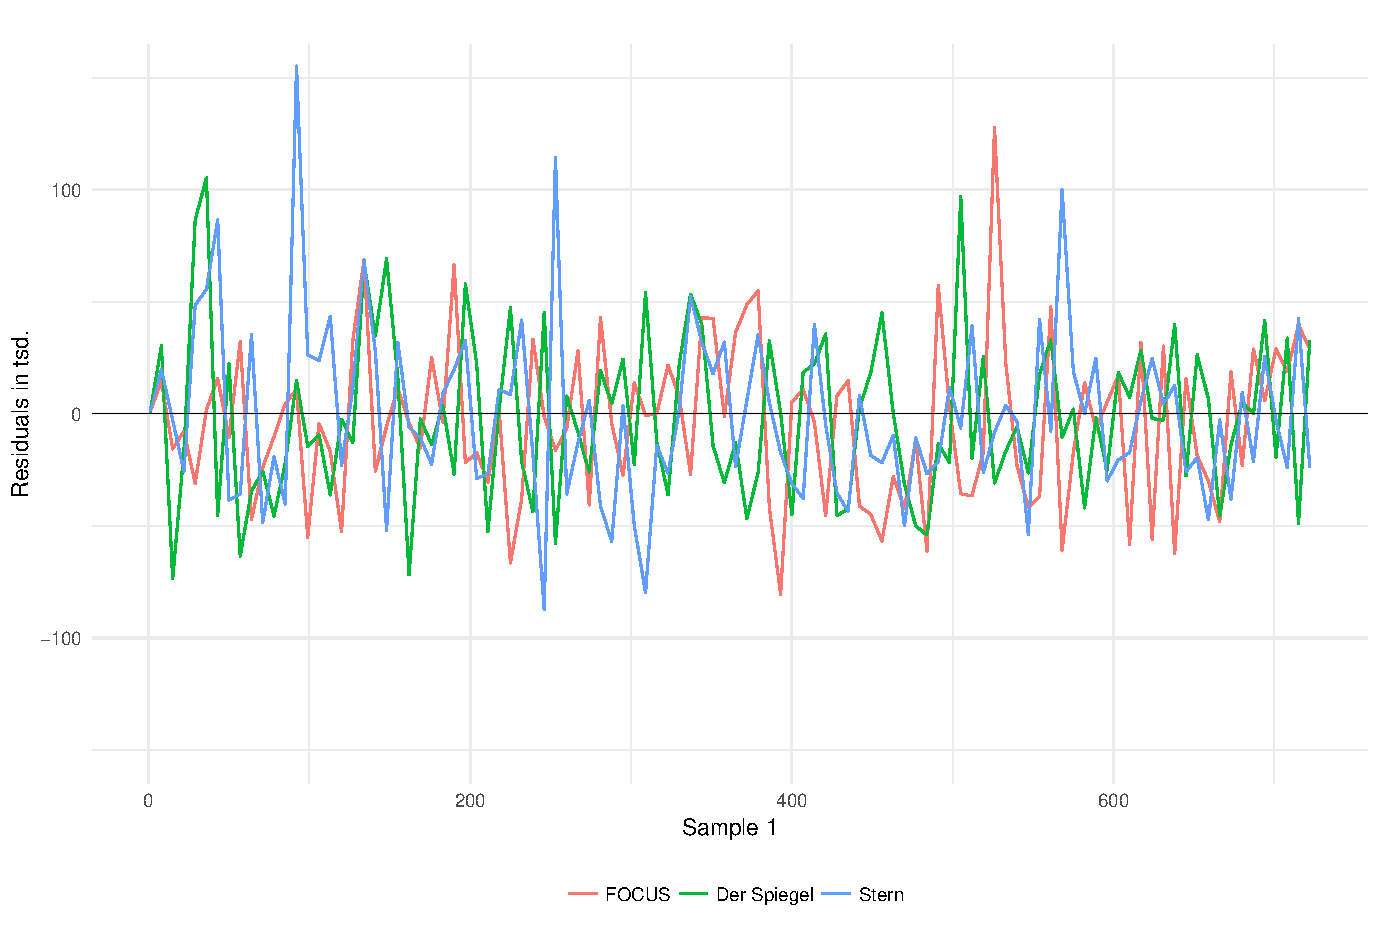
\includegraphics[scale=0.3]{../figs/arima_circ_fss1}}
		\subfloat[Sample 2]{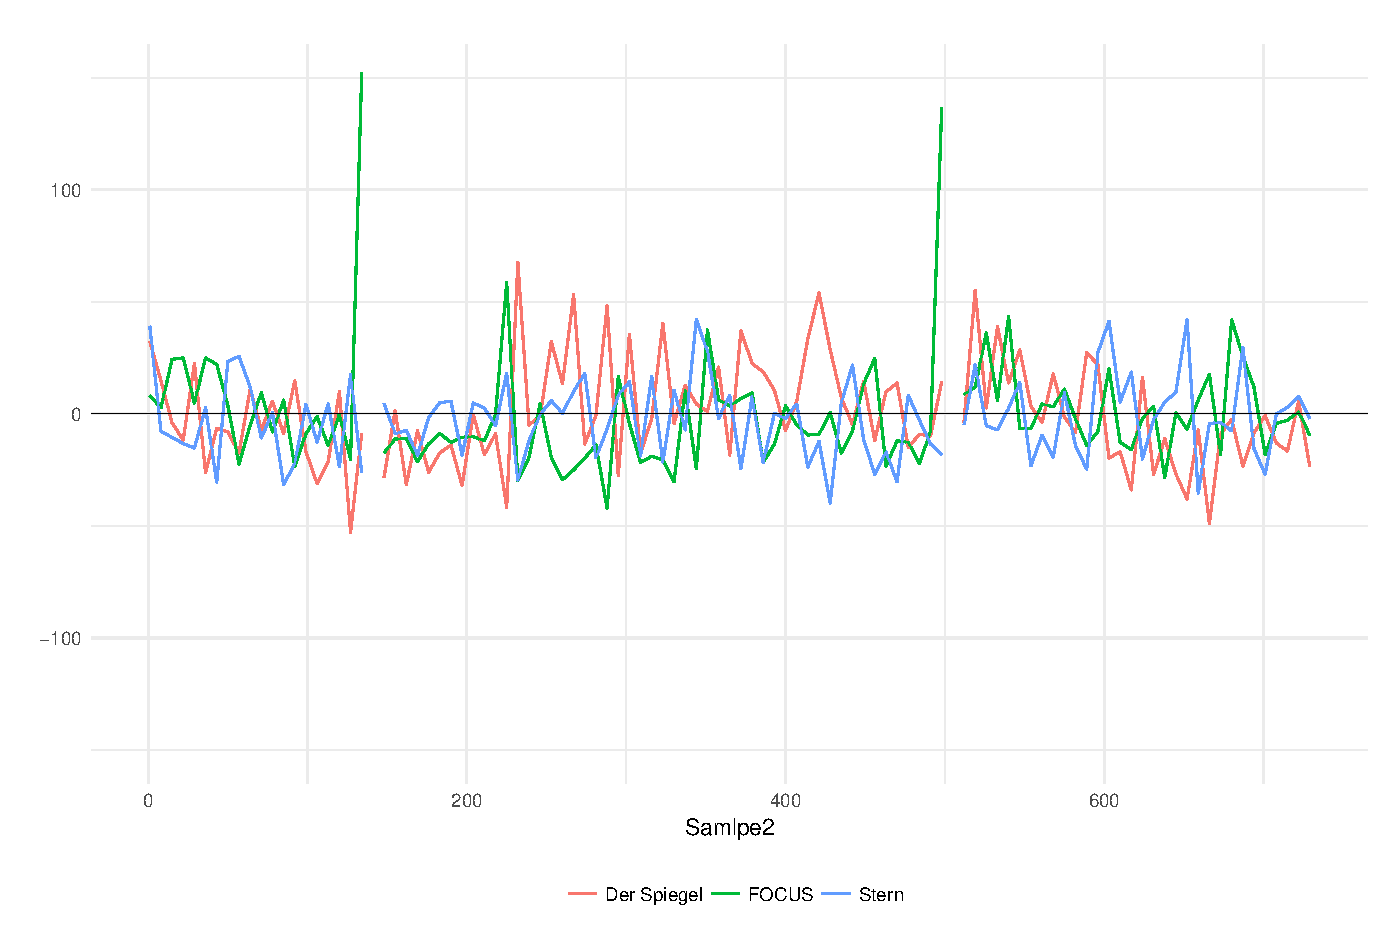
\includegraphics[scale=0.3]{../figs/arima_circ_fss2}}
		\label{fig_arima_sales_fss}
\end{figure}

\begin{figure}[H]
		\caption{Advertising pages of news magazines (adjusted)}
		\centering
		\subfloat[Sample 1]{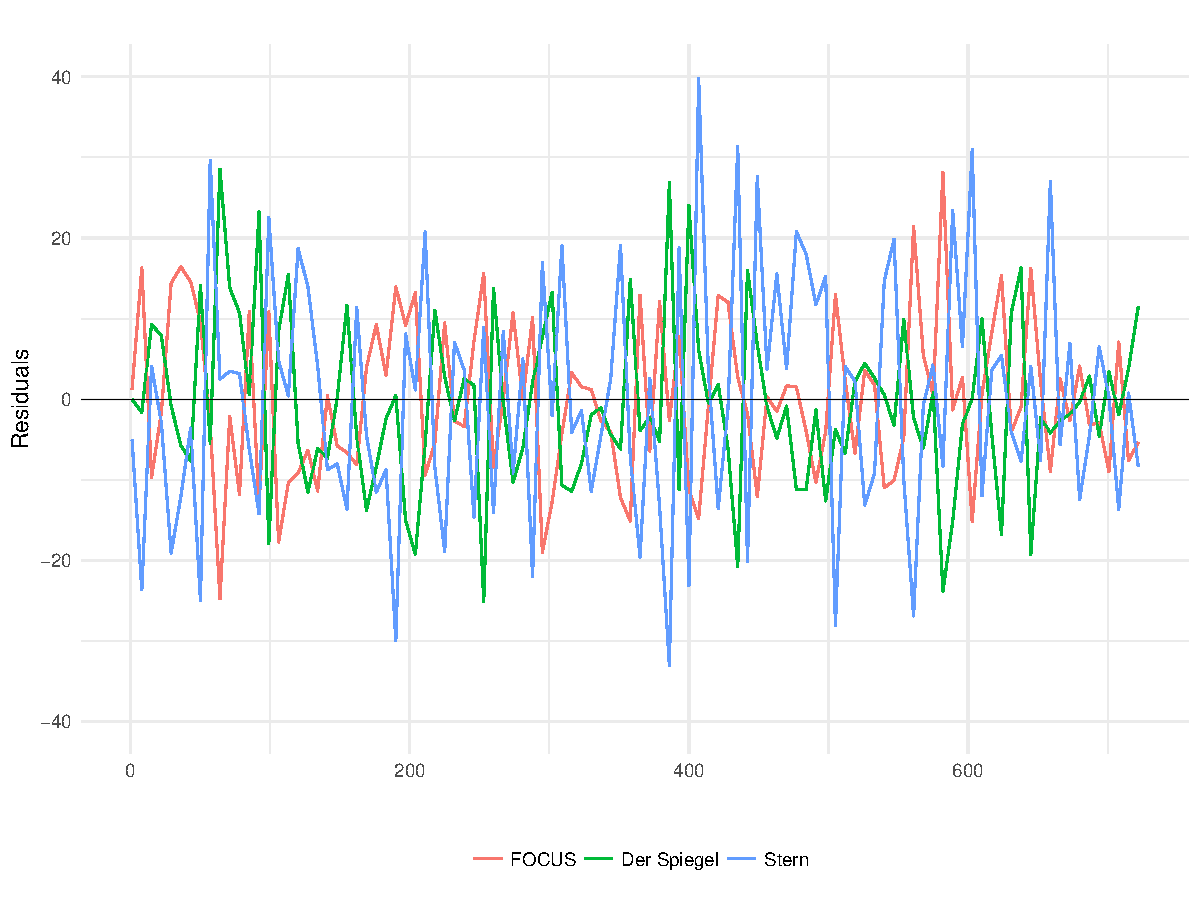
\includegraphics[scale=0.3]{../figs/arima_ads_fss1}}
		\subfloat[Sample 2]{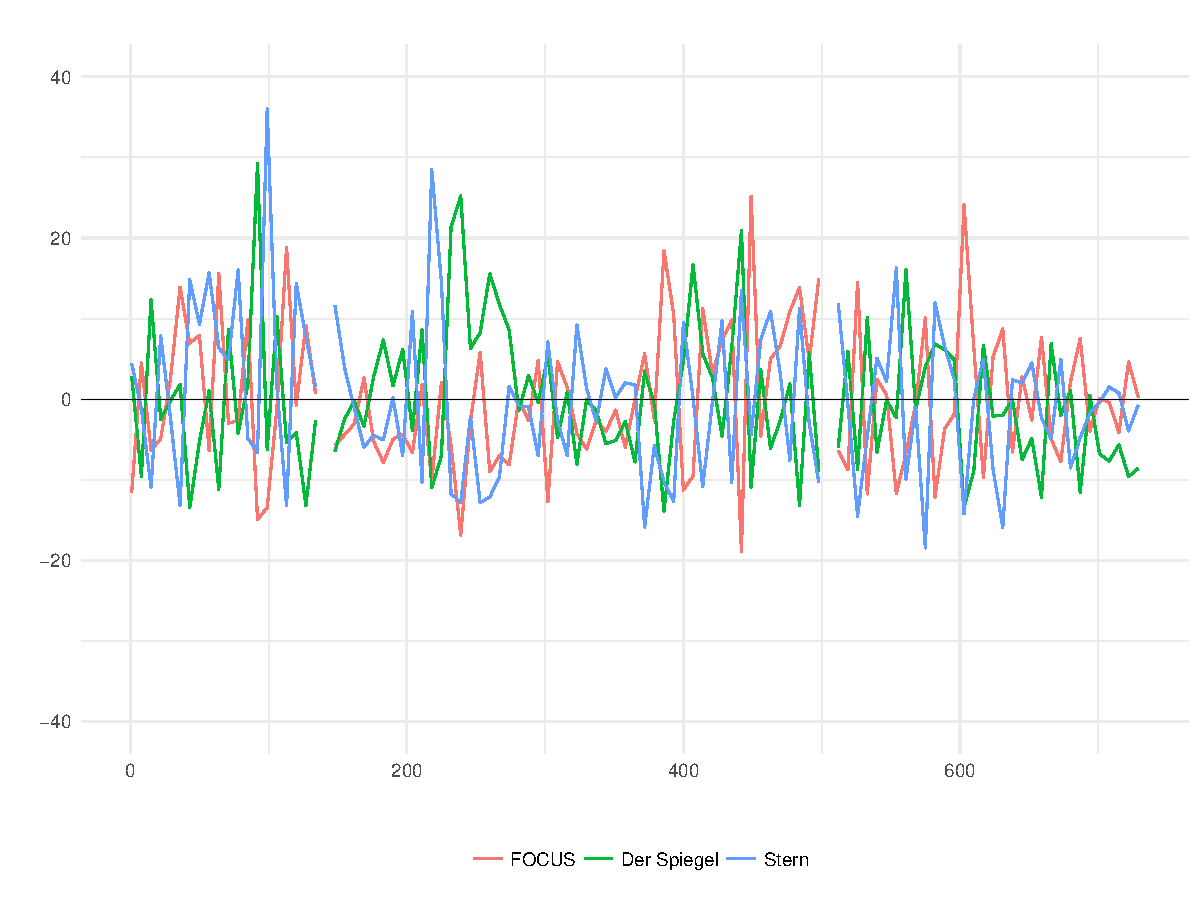
\includegraphics[scale=0.3]{../figs/arima_ads_fss2}}
		\label{fig_arima_ads_fss}
\end{figure}

\begin{figure}[H]
		\caption{Time Series of program guides (adjusted)}
		\centering
		\subfloat[Sales]{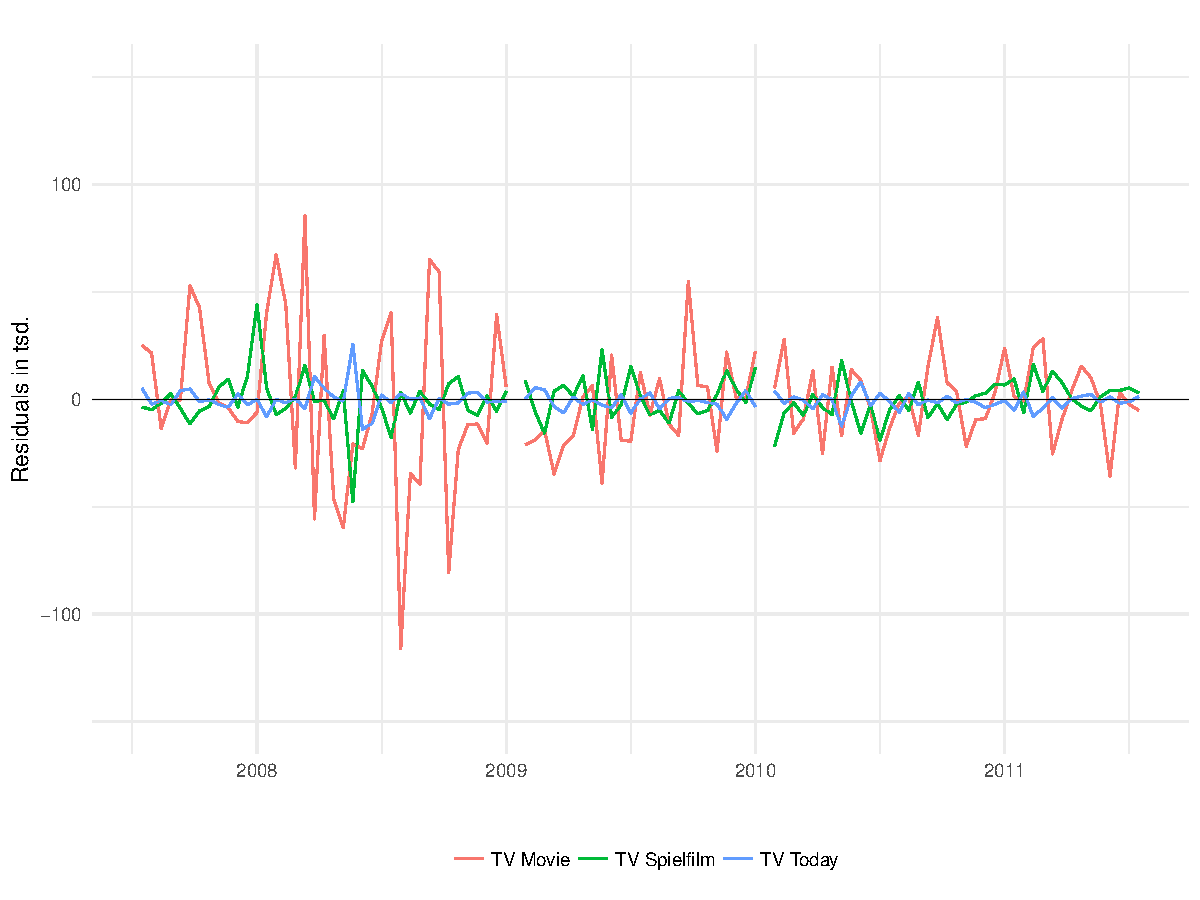
\includegraphics[scale=0.3]{../figs/arima_sales_tv}}
		\subfloat[Advertising Pages]{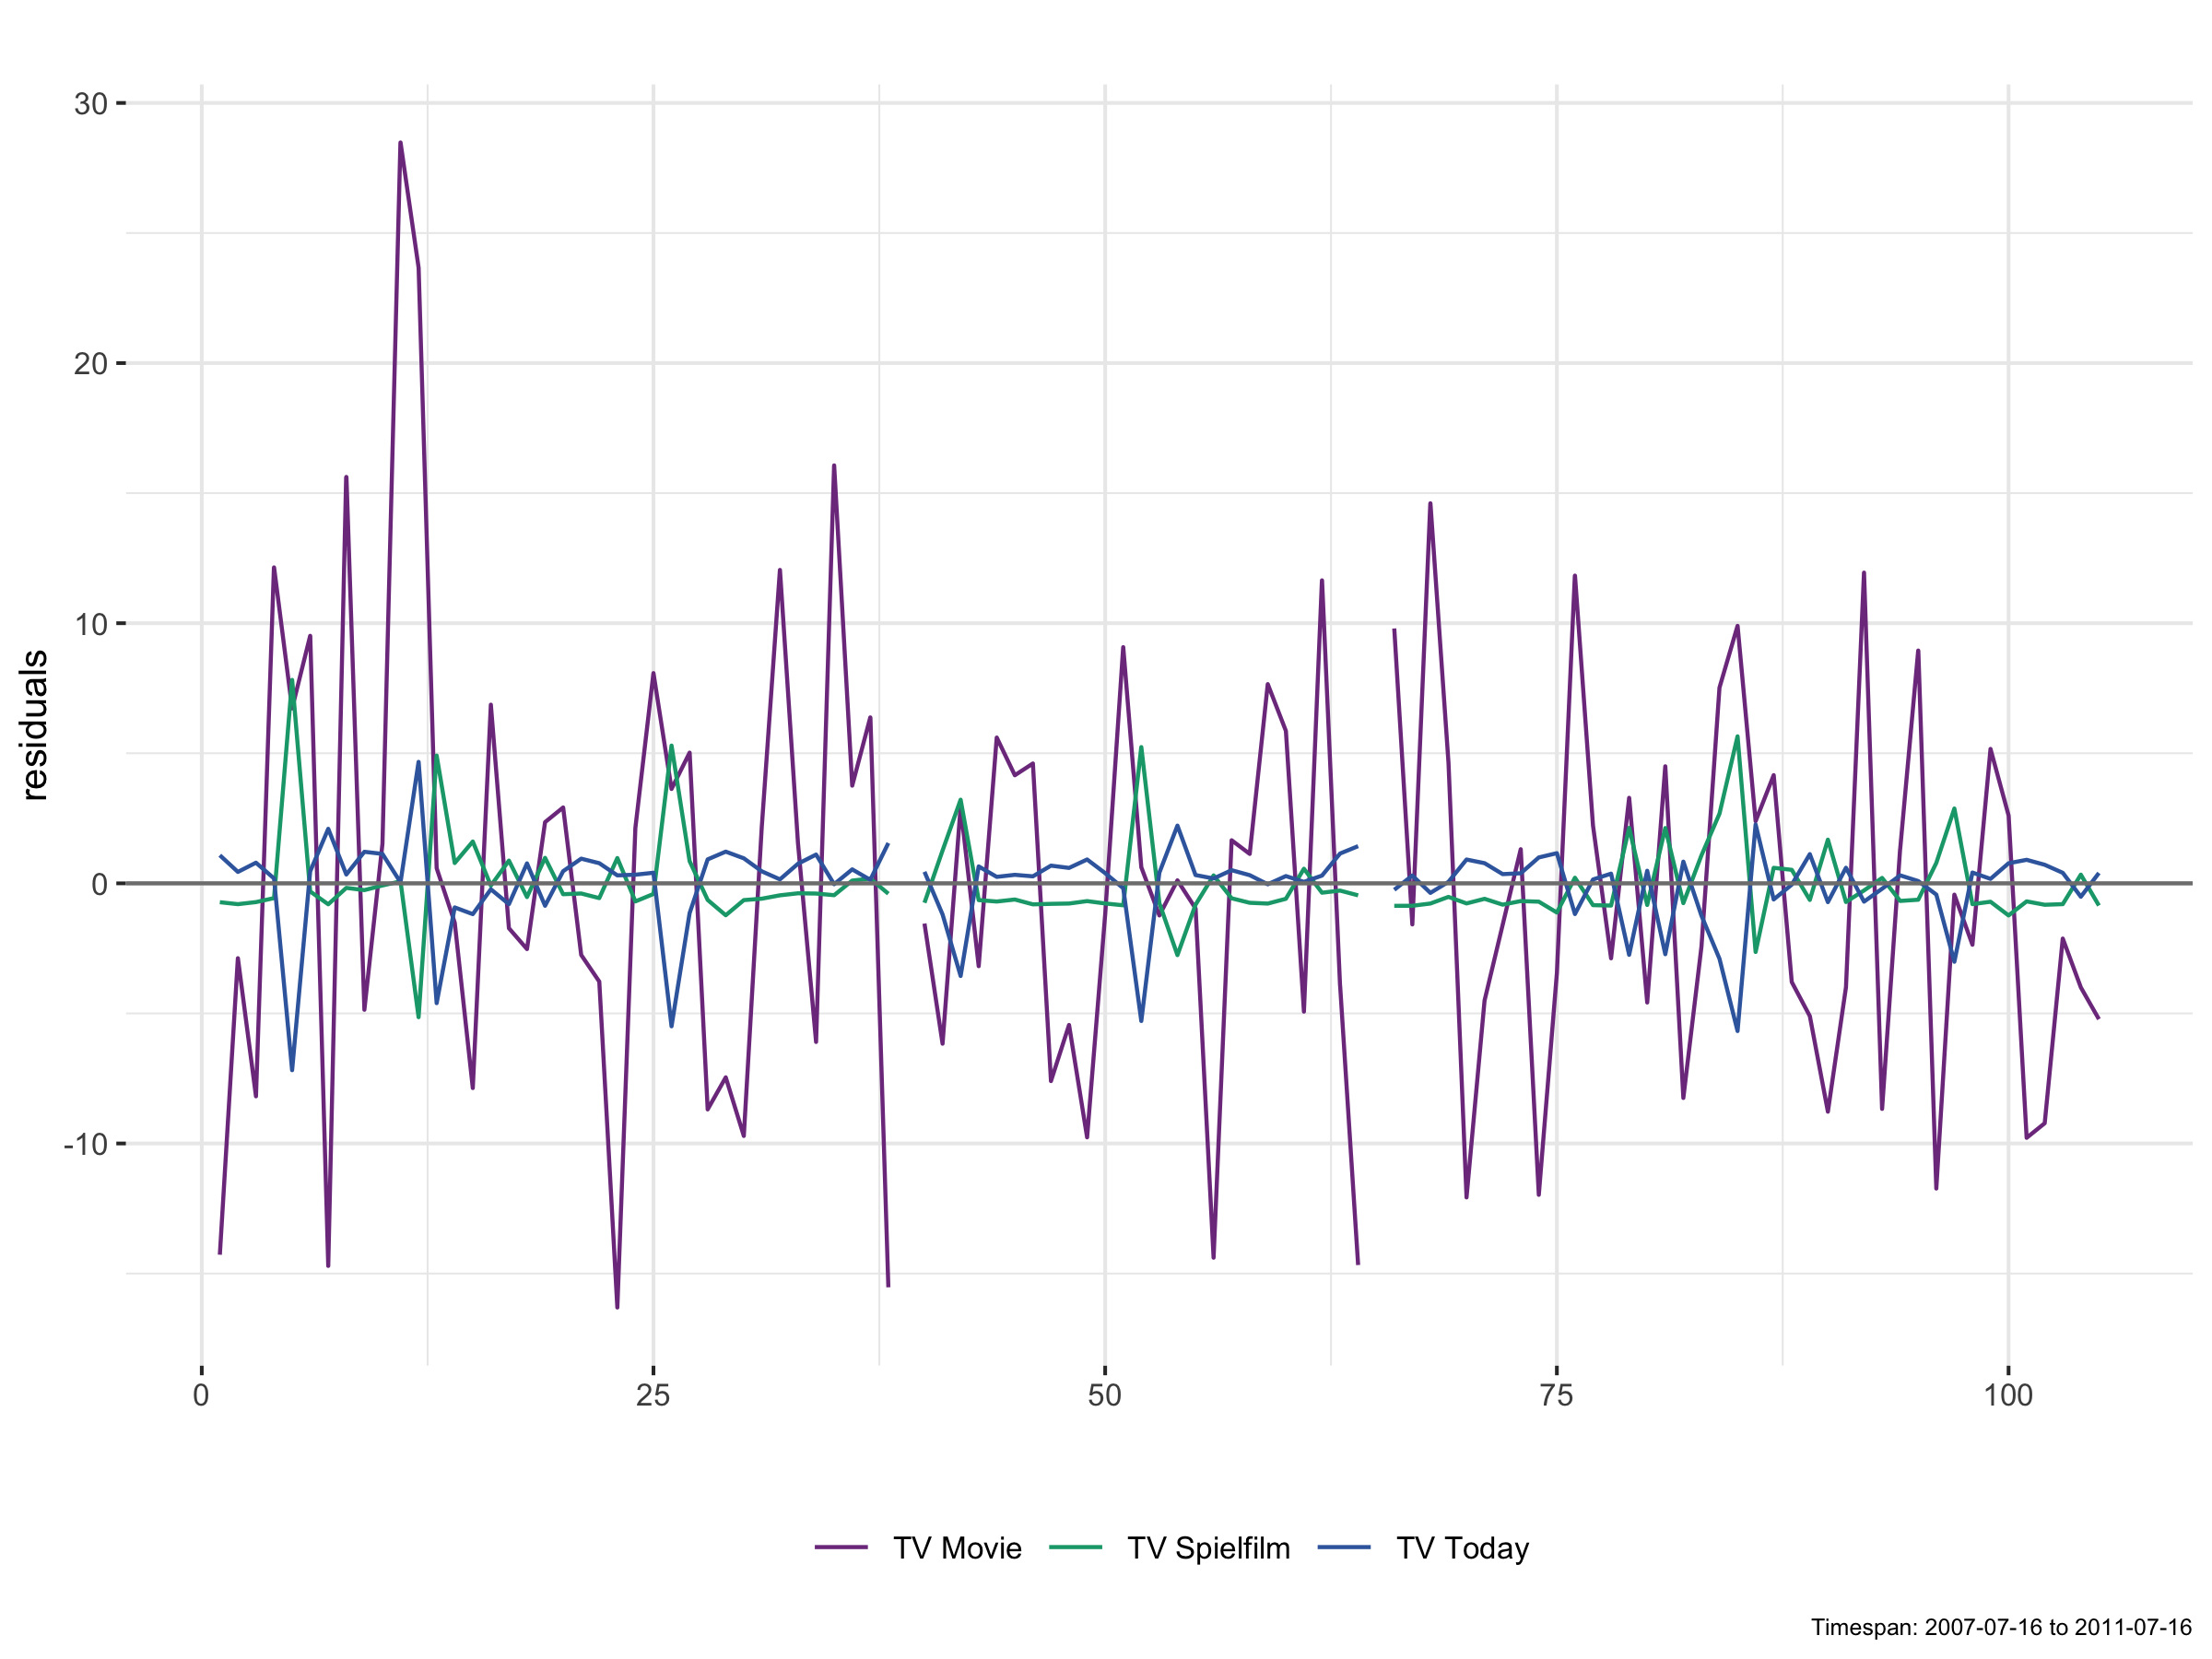
\includegraphics[scale=0.3]{../figs/arima_ads_tv}}
		\label{fig_arima_tv}
\end{figure}

\begin{figure}[H]
		\caption{Time Series of women magazines (adjusted)}
		\centering
		\subfloat[Sales]{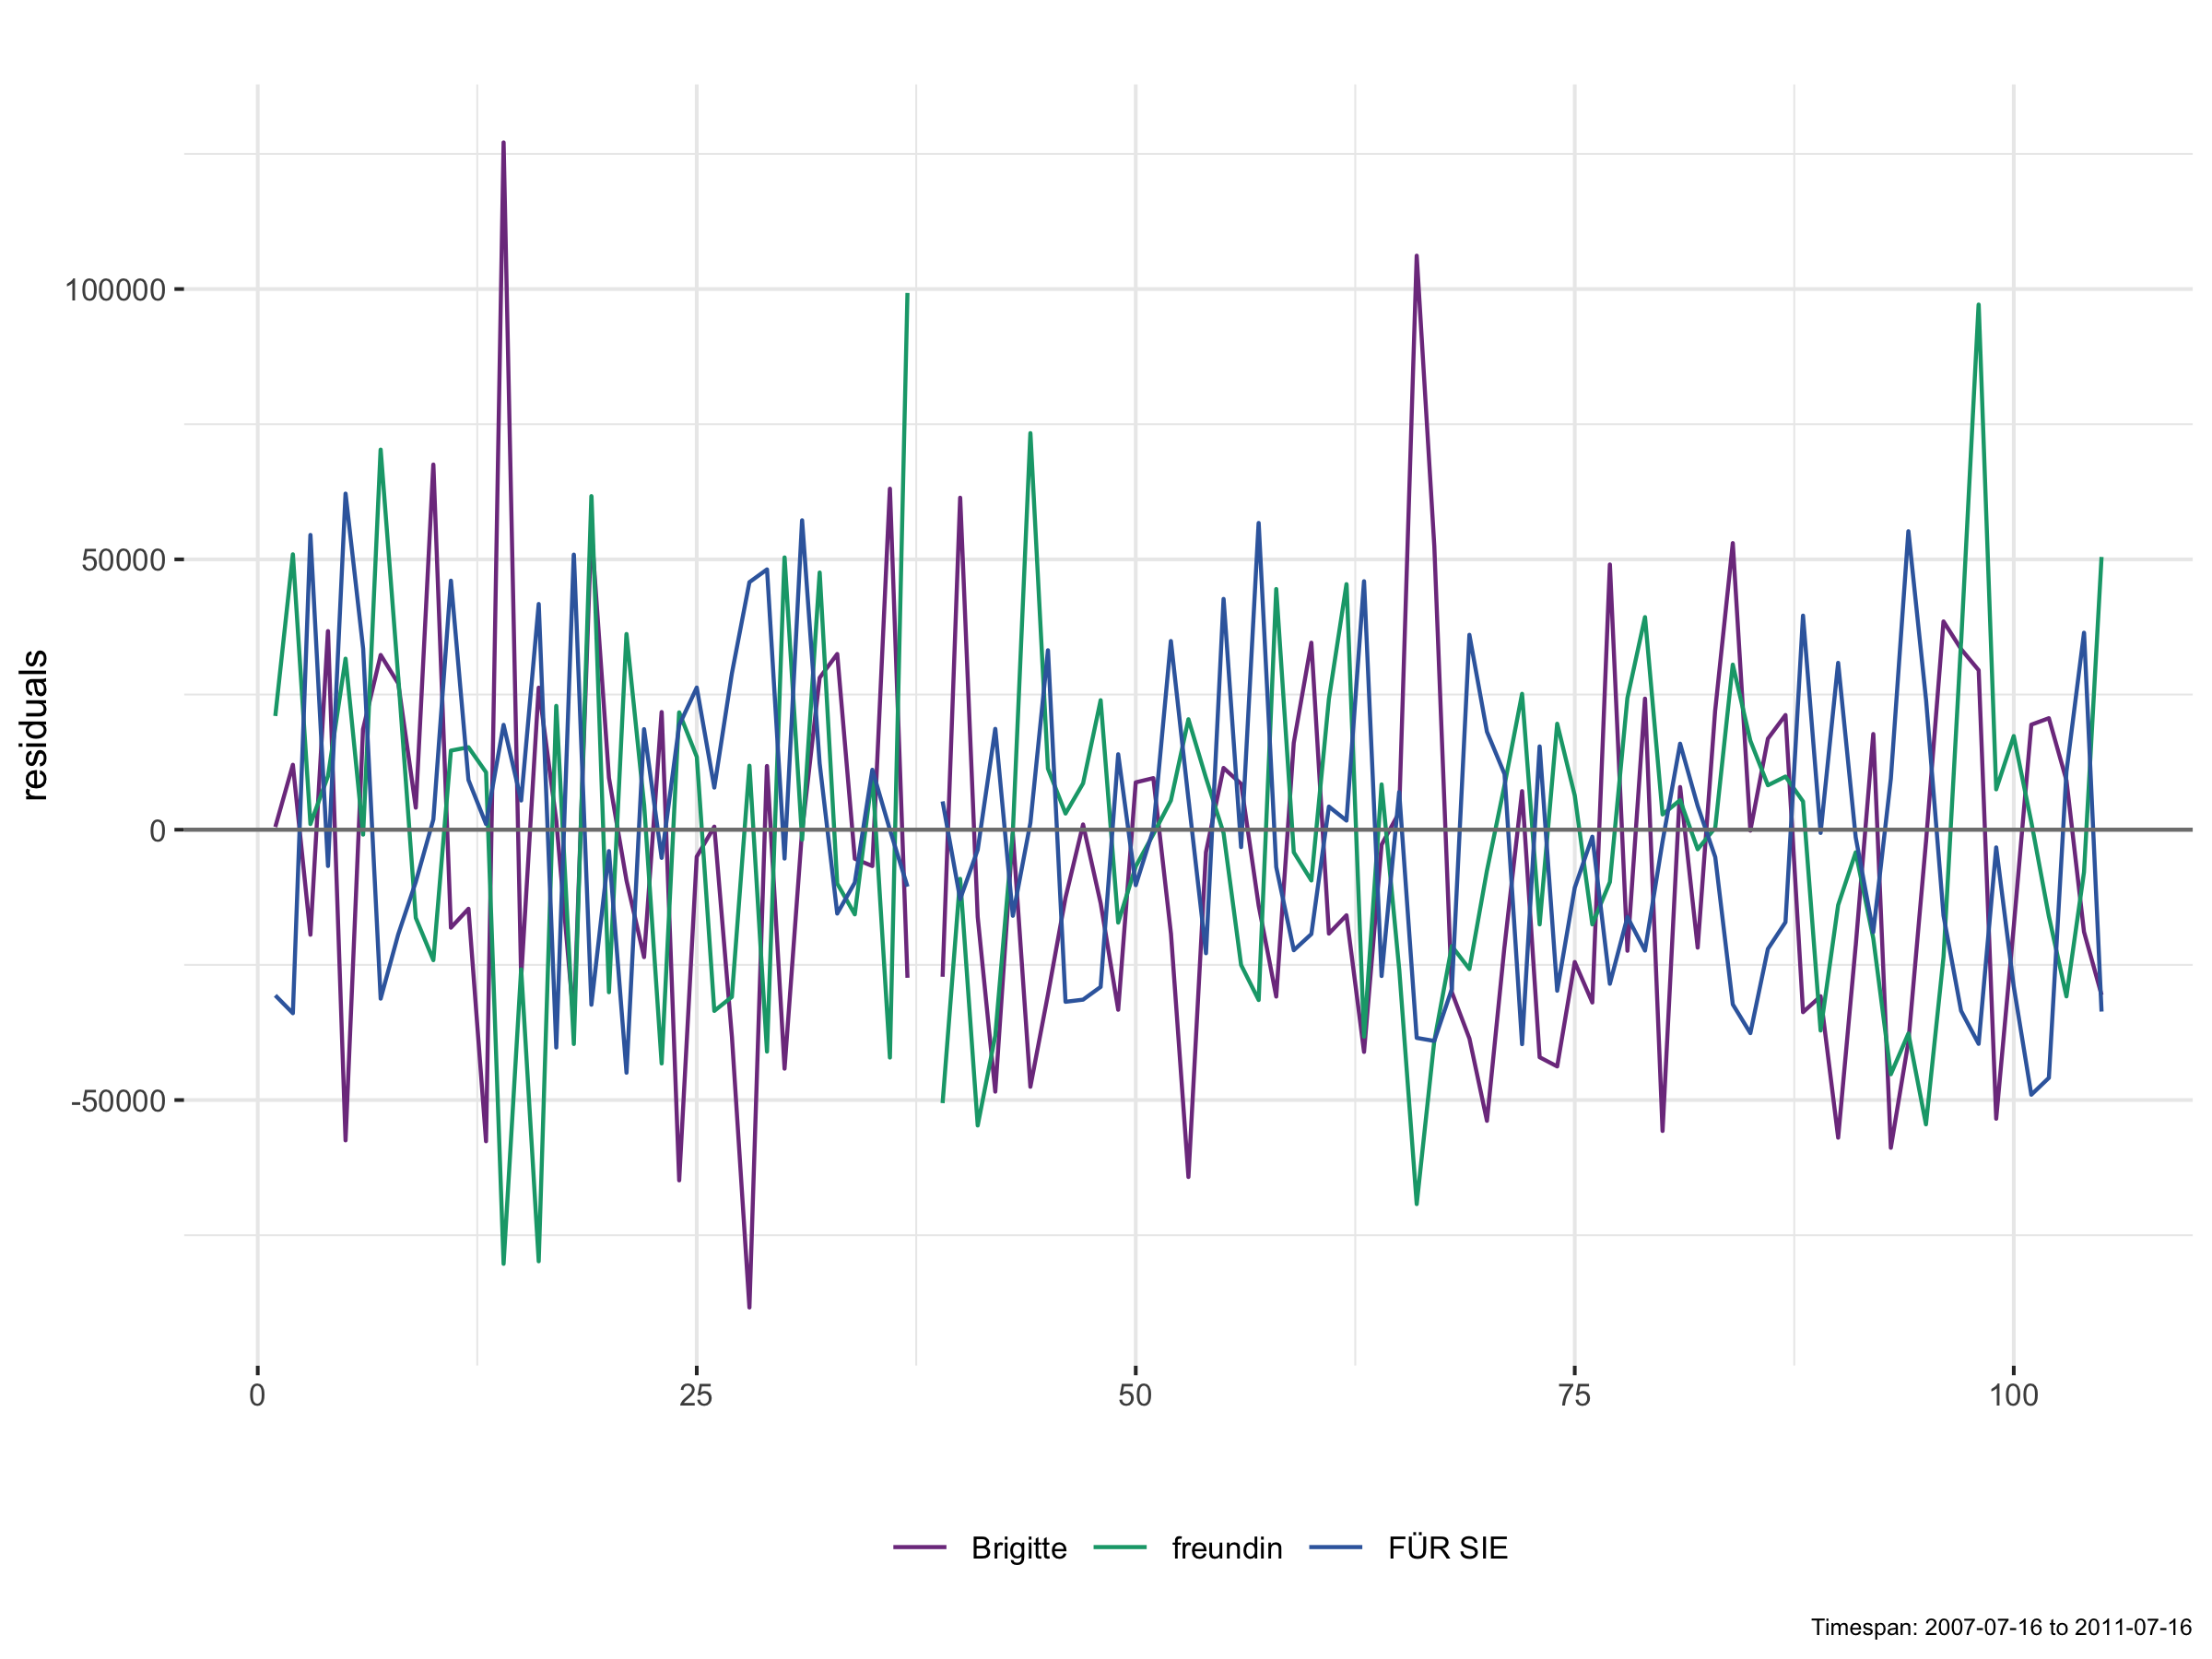
\includegraphics[scale=0.3]{../figs/arima_sales_women}}
		\subfloat[Advertising Pages]{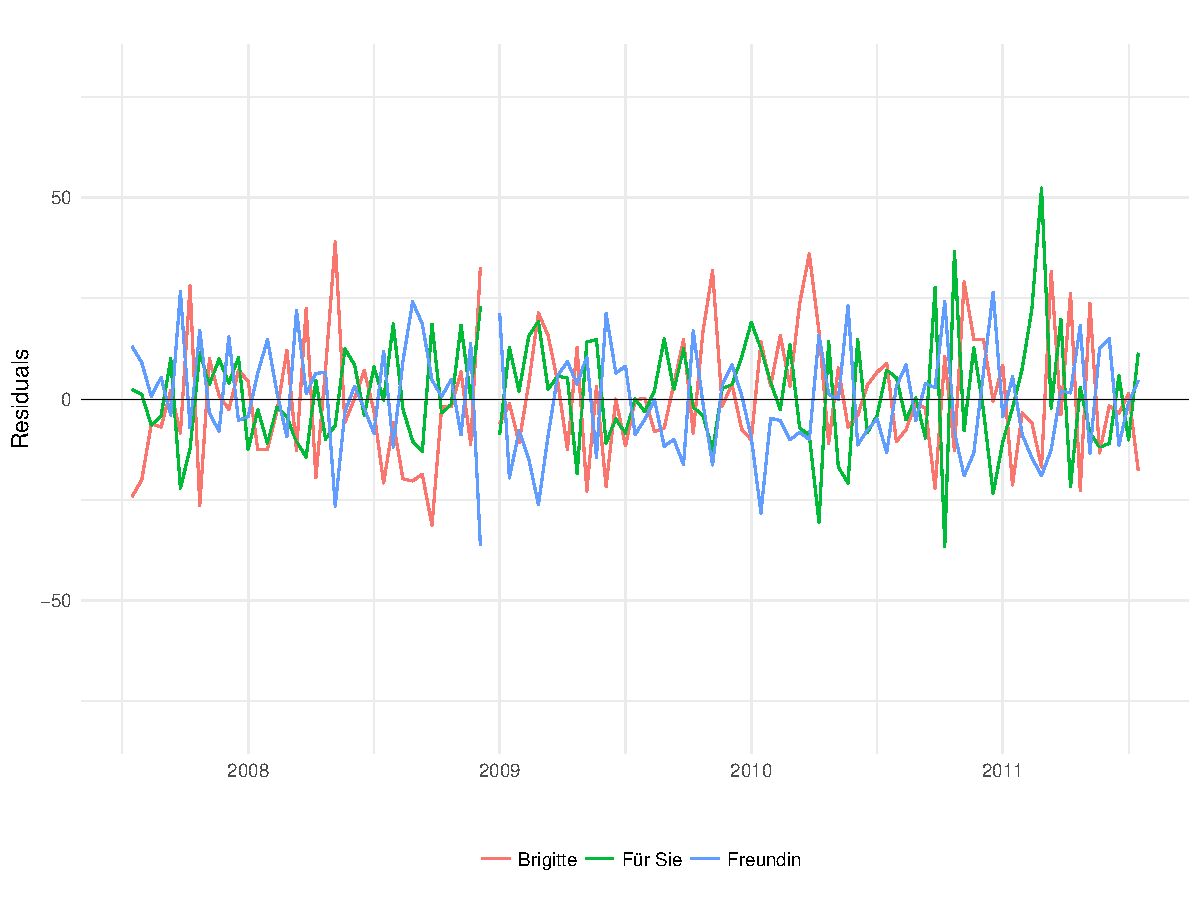
\includegraphics[scale=0.3]{../figs/arima_ads_women}}
		\label{fig_arima_women}
\end{figure}

\end{appendices}


\end{document}
